% Options for packages loaded elsewhere
% Options for packages loaded elsewhere
\PassOptionsToPackage{unicode}{hyperref}
\PassOptionsToPackage{hyphens}{url}
\PassOptionsToPackage{dvipsnames,svgnames,x11names}{xcolor}
%
\documentclass[
  letterpaper,
  DIV=11,
  numbers=noendperiod]{scrreprt}
\usepackage{xcolor}
\usepackage{amsmath,amssymb}
\setcounter{secnumdepth}{5}
\usepackage{iftex}
\ifPDFTeX
  \usepackage[T1]{fontenc}
  \usepackage[utf8]{inputenc}
  \usepackage{textcomp} % provide euro and other symbols
\else % if luatex or xetex
  \usepackage{unicode-math} % this also loads fontspec
  \defaultfontfeatures{Scale=MatchLowercase}
  \defaultfontfeatures[\rmfamily]{Ligatures=TeX,Scale=1}
\fi
\usepackage{lmodern}
\ifPDFTeX\else
  % xetex/luatex font selection
\fi
% Use upquote if available, for straight quotes in verbatim environments
\IfFileExists{upquote.sty}{\usepackage{upquote}}{}
\IfFileExists{microtype.sty}{% use microtype if available
  \usepackage[]{microtype}
  \UseMicrotypeSet[protrusion]{basicmath} % disable protrusion for tt fonts
}{}
\makeatletter
\@ifundefined{KOMAClassName}{% if non-KOMA class
  \IfFileExists{parskip.sty}{%
    \usepackage{parskip}
  }{% else
    \setlength{\parindent}{0pt}
    \setlength{\parskip}{6pt plus 2pt minus 1pt}}
}{% if KOMA class
  \KOMAoptions{parskip=half}}
\makeatother
% Make \paragraph and \subparagraph free-standing
\makeatletter
\ifx\paragraph\undefined\else
  \let\oldparagraph\paragraph
  \renewcommand{\paragraph}{
    \@ifstar
      \xxxParagraphStar
      \xxxParagraphNoStar
  }
  \newcommand{\xxxParagraphStar}[1]{\oldparagraph*{#1}\mbox{}}
  \newcommand{\xxxParagraphNoStar}[1]{\oldparagraph{#1}\mbox{}}
\fi
\ifx\subparagraph\undefined\else
  \let\oldsubparagraph\subparagraph
  \renewcommand{\subparagraph}{
    \@ifstar
      \xxxSubParagraphStar
      \xxxSubParagraphNoStar
  }
  \newcommand{\xxxSubParagraphStar}[1]{\oldsubparagraph*{#1}\mbox{}}
  \newcommand{\xxxSubParagraphNoStar}[1]{\oldsubparagraph{#1}\mbox{}}
\fi
\makeatother


\usepackage{longtable,booktabs,array}
\usepackage{calc} % for calculating minipage widths
% Correct order of tables after \paragraph or \subparagraph
\usepackage{etoolbox}
\makeatletter
\patchcmd\longtable{\par}{\if@noskipsec\mbox{}\fi\par}{}{}
\makeatother
% Allow footnotes in longtable head/foot
\IfFileExists{footnotehyper.sty}{\usepackage{footnotehyper}}{\usepackage{footnote}}
\makesavenoteenv{longtable}
\usepackage{graphicx}
\makeatletter
\newsavebox\pandoc@box
\newcommand*\pandocbounded[1]{% scales image to fit in text height/width
  \sbox\pandoc@box{#1}%
  \Gscale@div\@tempa{\textheight}{\dimexpr\ht\pandoc@box+\dp\pandoc@box\relax}%
  \Gscale@div\@tempb{\linewidth}{\wd\pandoc@box}%
  \ifdim\@tempb\p@<\@tempa\p@\let\@tempa\@tempb\fi% select the smaller of both
  \ifdim\@tempa\p@<\p@\scalebox{\@tempa}{\usebox\pandoc@box}%
  \else\usebox{\pandoc@box}%
  \fi%
}
% Set default figure placement to htbp
\def\fps@figure{htbp}
\makeatother





\setlength{\emergencystretch}{3em} % prevent overfull lines

\providecommand{\tightlist}{%
  \setlength{\itemsep}{0pt}\setlength{\parskip}{0pt}}



 


\KOMAoption{captions}{tableheading}
\makeatletter
\@ifpackageloaded{bookmark}{}{\usepackage{bookmark}}
\makeatother
\makeatletter
\@ifpackageloaded{caption}{}{\usepackage{caption}}
\AtBeginDocument{%
\ifdefined\contentsname
  \renewcommand*\contentsname{Table of contents}
\else
  \newcommand\contentsname{Table of contents}
\fi
\ifdefined\listfigurename
  \renewcommand*\listfigurename{List of Figures}
\else
  \newcommand\listfigurename{List of Figures}
\fi
\ifdefined\listtablename
  \renewcommand*\listtablename{List of Tables}
\else
  \newcommand\listtablename{List of Tables}
\fi
\ifdefined\figurename
  \renewcommand*\figurename{Figure}
\else
  \newcommand\figurename{Figure}
\fi
\ifdefined\tablename
  \renewcommand*\tablename{Table}
\else
  \newcommand\tablename{Table}
\fi
}
\@ifpackageloaded{float}{}{\usepackage{float}}
\floatstyle{ruled}
\@ifundefined{c@chapter}{\newfloat{codelisting}{h}{lop}}{\newfloat{codelisting}{h}{lop}[chapter]}
\floatname{codelisting}{Listing}
\newcommand*\listoflistings{\listof{codelisting}{List of Listings}}
\makeatother
\makeatletter
\makeatother
\makeatletter
\@ifpackageloaded{caption}{}{\usepackage{caption}}
\@ifpackageloaded{subcaption}{}{\usepackage{subcaption}}
\makeatother
\usepackage{bookmark}
\IfFileExists{xurl.sty}{\usepackage{xurl}}{} % add URL line breaks if available
\urlstyle{same}
\hypersetup{
  pdftitle={Portofolio},
  pdfauthor={Muhammad Reyna Athallah Agoes},
  colorlinks=true,
  linkcolor={blue},
  filecolor={Maroon},
  citecolor={Blue},
  urlcolor={Blue},
  pdfcreator={LaTeX via pandoc}}


\title{Portofolio}
\usepackage{etoolbox}
\makeatletter
\providecommand{\subtitle}[1]{% add subtitle to \maketitle
  \apptocmd{\@title}{\par {\large #1 \par}}{}{}
}
\makeatother
\subtitle{Portfolio Asesmen II-2100 KIPP}
\author{Muhammad Reyna Athallah Agoes}
\date{2025-10-31}
\begin{document}
\maketitle

\renewcommand*\contentsname{Table of contents}
{
\hypersetup{linkcolor=}
\setcounter{tocdepth}{2}
\tableofcontents
}

\bookmarksetup{startatroot}

\chapter*{Selamat Berjumpa}\label{selamat-berjumpa}
\addcontentsline{toc}{chapter}{Selamat Berjumpa}

\markboth{Selamat Berjumpa}{Selamat Berjumpa}

\includegraphics[width=1\linewidth,height=\textheight,keepaspectratio]{images/muka_gw.jpg}

Perkenalkan , Muhammad Reyna Athallah Agoes mahasiswa di Sekolah Teknik
Elektro dan Informatika.ITB angkatan 2024.

\textbf{``Sayangi Orang Sekitarmu dan Maknai Hidup Lebih Dalam''}

\bookmarksetup{startatroot}

\chapter{UTS-1 All About Me}\label{uts-1-all-about-me}

\begin{figure}[H]

{\centering \includegraphics[width=9.5\linewidth,height=\textheight,keepaspectratio]{All_About_me/../images/AZRL.png}

}

\caption{About Me}

\end{figure}%

Armein Z R Langi adalah Guru Besar di Sekolah Teknik Elektro dan
Informatika ITB, dosen ITB sejak Desember 1987, mantan Rektor
Universitas Kristen Maranatha, 1 Maret 2016 s/d 29 Februari 2020, mantan
Kepala Pusat Penelitian Teknologi Informasi dan Komunikasi (PP-TIK) ITB
November 2005 s/d Maret 2010, dan Sekretaris MWA ITB Mei 2010-Jan 2011.

Lahir di Tomohon 1962 dari pasangan Manado dan Sunda. Saat ini tinggal
di Bandung, menikah dengan Ina dan dikaruniai empat anak. Ayah dari
Gladys, Kezia, Andria, dan Marco.

Sharing pikiran singkat ada di blog \url{https://azrl.wordpress.com}.
Facebookk: armein\_langi

Apa gagasan yang sedang ia pikirkan?

\section{\texorpdfstring{\textbf{Kisah yang Membentuk Diri Anda:
Mengenal Kekuatan Identitas
Naratif}}{Kisah yang Membentuk Diri Anda: Mengenal Kekuatan Identitas Naratif}}\label{kisah-yang-membentuk-diri-anda-mengenal-kekuatan-identitas-naratif}

Manusia adalah pencerita alami. Sejak zaman dahulu, kita selalu berusaha
memahami kekacauan hidup dengan merangkainya menjadi sebuah cerita. Para
ahli bahkan menyebut kita sebagai ``organisme pencerita''
(\emph{storytelling organisms}) yang menjalani ``kehidupan yang penuh
cerita'' (\emph{storied lives}) (2). Proses ini bukanlah sekadar
menyusun fakta, melainkan sebuah proses aktif untuk menciptakan makna.

\href{./audio/Identitas_Naratif__Jadi_Sutradara_dan_Penulis_Kisah_Hidup_Anda_.mp4}{Hayu
dengar poscastnya}

Kisah personal yang terus berkembang inilah yang disebut para psikolog
sebagai \textbf{``identitas naratif''}---sebuah cerita yang kita bangun
untuk memahami keberadaan kita, dengan menghubungkan masa lalu, masa
kini, dan masa depan kita menjadi satu kesatuan yang utuh (3, 8). Cerita
batin ini adalah proses \emph{penciptaan diri} yang aktif, bukan sekadar
menceritakan ulang kejadian. Kisah inilah yang menjawab
pertanyaan-pertanyaan paling mendasar: ``Siapa saya? Bagaimana saya
sampai di sini? Ke mana saya akan pergi?'' (5, 6).

\subsection{\texorpdfstring{\textbf{1. Tiga Lapisan Diri Anda: Di Mana
Cerita Hidup Anda
Berada?}}{1. Tiga Lapisan Diri Anda: Di Mana Cerita Hidup Anda Berada?}}\label{tiga-lapisan-diri-anda-di-mana-cerita-hidup-anda-berada}

Psikolog Dan P. McAdams membagi kepribadian manusia ke dalam tiga
tingkatan yang berbeda. Identitas naratif merupakan tingkatan tertinggi
dan paling personal, yang menyatukan semua bagian lain dari diri kita
(8).

\begin{itemize}
\item
  \textbf{Level 1: Sifat Dasar} Ini adalah ciri-ciri umum kepribadian
  kita yang cenderung stabil, seperti apakah kita seorang
  \emph{introvert} atau \emph{ekstrovert}.
\item
  \textbf{Level 2: Kepedulian Pribadi} Ini mencakup hal-hal yang lebih
  spesifik seperti tujuan hidup, nilai-nilai yang kita pegang, dan
  keyakinan kita.
\item
  \textbf{Level 3: Identitas Naratif} Inilah kisah hidup yang kita
  ciptakan untuk mengikat Level 1 dan 2 menjadi sebuah narasi yang
  koheren dan bermakna. Ini adalah cerita tentang ``diri'' kita.
\end{itemize}

Wawasan paling memberdayakan dari konsep ini adalah: meskipun kita
mungkin tidak dapat dengan mudah mengubah sifat dasar kita (Level 1),
kita \emph{memiliki kekuatan} untuk belajar mengubah cerita yang kita
sampaikan tentang hidup kita (Level 3). Perubahan narasi ini terbukti
memiliki dampak besar pada kesejahteraan dan kebahagiaan kita (9).

Namun, tidak semua cerita diciptakan sama. Mari kita lihat pola-pola
naratif yang dapat membuat sebuah kisah hidup menjadi lebih
memberdayakan.

\subsection{\texorpdfstring{\textbf{2. Pola-Pola Kisah Kehidupan: Apa
yang Membuat Sebuah Cerita
Bermanfaat?}}{2. Pola-Pola Kisah Kehidupan: Apa yang Membuat Sebuah Cerita Bermanfaat?}}\label{pola-pola-kisah-kehidupan-apa-yang-membuat-sebuah-cerita-bermanfaat}

Penelitian menunjukkan bahwa tidak semua cerita yang kita bangun
sama-sama bermanfaat bagi kesehatan mental kita (4). Beberapa tema
naratif secara konsisten terhubung dengan kehidupan yang lebih sejahtera
dan berkembang.

\subsubsection{Penebusan vs.~Kontaminasi: Mengubah Penderitaan Menjadi
Kekuatan}\label{penebusan-vs.-kontaminasi-mengubah-penderitaan-menjadi-kekuatan}

Salah satu pola naratif yang paling penting adalah cara kita membingkai
peristiwa sulit.

\textbf{Cerita Penebusan (Redemption Story)} adalah narasi yang bergerak
dari situasi negatif ke hasil yang positif (misalnya, kegagalan yang
memberikan pelajaran berharga, atau penderitaan yang melahirkan kekuatan
baru). Pola ini sangat kuat kaitannya dengan kebahagiaan, kepuasan
hidup, dan resiliensi (7).

\textbf{Cerita Kontaminasi (Contamination Story)} adalah kebalikannya.
Cerita ini dimulai dari peristiwa baik yang kemudian berubah menjadi
buruk. Kisah semacam ini seperti ``tumpahan minyak yang meracuni air,''
menjebak sang pencerita dalam rasa sakit dan putus asa (3, 11).

\subsubsection{Agensi vs.~Kepasifan: Menjadi Pahlawan dalam Kisah
Anda}\label{agensi-vs.-kepasifan-menjadi-pahlawan-dalam-kisah-anda}

Pola penting lainnya adalah peran yang kita ambil dalam cerita kita
sendiri.

\textbf{Agensi (Agency)} adalah ketika kita menampilkan diri sebagai
aktor utama dalam cerita kita---seseorang yang secara aktif membuat
keputusan, mengambil tindakan, dan mengatasi rintangan. Mengembangkan
rasa agensi dalam cerita hidup adalah salah satu prediktor terkuat untuk
perbaikan dalam terapi (3, 7).

\textbf{Kepasifan (Passivity)} ditandai dengan perasaan menjadi korban
keadaan. Dalam narasi ini, peristiwa seolah-olah ``terjadi begitu saja
pada'' sang pencerita, yang digambarkan sebagai korban pasif dari takdir
atau tindakan orang lain (8).

Tabel berikut merangkum tema-tema naratif yang membangun dan merusak,
beserta dampaknya bagi kesejahteraan kita.

\begin{longtable}[]{@{}
  >{\raggedright\arraybackslash}p{(\linewidth - 2\tabcolsep) * \real{0.5000}}
  >{\raggedright\arraybackslash}p{(\linewidth - 2\tabcolsep) * \real{0.5000}}@{}}
\toprule\noalign{}
\endhead
\bottomrule\noalign{}
\endlastfoot
Pola Naratif & Dampak Psikologis \\
\textbf{Pola Naratif yang Membangun (Generative Themes)} & \\
\textbf{Penebusan} (Negatif → Positif) & Meningkatkan kebahagiaan,
kepuasan hidup, resiliensi, dan \emph{generativitas} (keinginan untuk
berkontribusi pada kesejahteraan generasi mendatang) (4, 7). \\
\textbf{Agensi} (Diri sebagai Aktor Efektif) & Meningkatkan kepercayaan
diri, kesehatan mental, dan merupakan prediktor kuat perbaikan dalam
terapi (7). \\
\textbf{Koneksi} (Hubungan \& Rasa Memiliki) & Meningkatkan
kesejahteraan, mengurangi rasa kesepian, dan memberikan rasa memiliki
tujuan hidup yang lebih besar (8). \\
\textbf{Pola Naratif yang Merusak (Disruptive Themes)} & \\
\textbf{Kontaminasi} (Positif → Negatif) & Menurunkan kesejahteraan,
menyebabkan depresi, keputusasaan, dan perasaan terperangkap dalam
pengalaman negatif (3). \\
\textbf{Kepasifan} (Diri sebagai Korban) & Menimbulkan perasaan menjadi
korban, demotivasi, rasa tidak berdaya, depresi, dan hasil kesehatan
mental yang buruk (8). \\
\textbf{Isolasi} (Terputus dari Orang Lain) & Menyebabkan kesepian,
keputusasaan, kurangnya dukungan sosial, dan meningkatkan kerentanan
terhadap gangguan psikologis (8). \\
\end{longtable}

Lalu, bagaimana pikiran kita menciptakan pola-pola naratif ini?
Jawabannya terletak pada sebuah proses kognitif yang luar biasa.

\subsection{\texorpdfstring{\textbf{3. Seni Memberi Makna: Kekuatan
Super Anda dalam
Bernalar}}{3. Seni Memberi Makna: Kekuatan Super Anda dalam Bernalar}}\label{seni-memberi-makna-kekuatan-super-anda-dalam-bernalar}

Pikiran kita memiliki ``mesin pembuat makna'' yang disebut
\textbf{penalaran otobiografis} (\emph{autobiographical reasoning}).
Inilah kemampuan kognitif yang memungkinkan kita menghubungkan
peristiwa-peristiwa dalam hidup dengan identitas diri kita dan memahami
signifikansinya (10).

Tanpa penalaran ini, hidup kita hanyalah daftar kejadian. Dengan
penalaran ini, hidup kita menjadi sebuah cerita yang bermakna.

Temuan paling penting dari psikologi naratif adalah ini:
\textbf{kemampuan kita untuk memaknai peristiwa sulit secara positif
(misalnya, menemukan hikmah atau pelajaran) lebih berpengaruh pada
kesejahteraan kita daripada peristiwa itu sendiri} (10). Ini bukan sifat
bawaan, melainkan sebuah keterampilan yang bisa dipelajari dan dilatih.

Memahami hal ini memberi kita kekuatan. Langkah-langkah berikutnya
adalah latihan praktis untuk mengasah `mesin pembuat makna' ini dan
menjadi penulis yang lebih sadar atas kisah hidup kita sendiri.

\subsection{\texorpdfstring{\textbf{4. Mulai Menulis Ulang Kisah Anda:
Dua Langkah
Praktis}}{4. Mulai Menulis Ulang Kisah Anda: Dua Langkah Praktis}}\label{mulai-menulis-ulang-kisah-anda-dua-langkah-praktis}

Meskipun kita tidak bisa mengubah masa lalu, kita memiliki kekuatan luar
biasa untuk mengubah \emph{cerita} yang kita sampaikan tentang masa lalu
itu (29). Berikut adalah dua langkah praktis yang terinspirasi dari
Terapi Naratif untuk memulai proses ini.

\subsubsection{Langkah 1: Pisahkan Diri Anda dari
Masalah}\label{langkah-1-pisahkan-diri-anda-dari-masalah}

Teknik ini disebut \textbf{eksternalisasi masalah}. Caranya adalah
dengan mengubah cara kita berbicara tentang masalah kita.

Misalnya, alih-alih berpikir, \emph{``Saya adalah orang yang
pencemas,''} coba bingkai ulang menjadi, \emph{``Saya adalah orang yang
sedang berhadapan dengan pengaruh kecemasan''} (35).

Pergeseran bahasa yang sederhana ini menciptakan jarak psikologis.
Masalah tidak lagi menjadi bagian inti dari identitas Anda, melainkan
sesuatu di luar diri Anda yang bisa diamati, dipahami, dan dihadapi. Ini
membuat masalah terasa jauh lebih bisa dikelola.

\subsubsection{Langkah 2: Temukan ``Momen Berkilau''
Anda}\label{langkah-2-temukan-momen-berkilau-anda}

Setelah Anda memisahkan diri dari masalah, langkah selanjutnya adalah
mencari bukti yang bertentangan dengan ``cerita yang penuh masalah''
tersebut. Dalam Terapi Naratif, ini disebut \emph{unique outcomes} atau
yang bisa kita sebut \textbf{momen berkilau} (\emph{sparkling moments}).

Ini adalah momen-momen, sekecil apa pun, di mana masalah tersebut tidak
berkuasa atas diri Anda. Tanyakan pada diri Anda:

``Ingatkah saat di mana `Si Pengkritik' dalam diri Anda muncul, tetapi
Anda tetap berhasil bertindak dengan percaya diri?'' (36)

Atau, ``Apakah ada momen ketika `rasa malas' mencoba mengambil alih,
tetapi Anda tetap berhasil menyelesaikan tugas itu?''

Momen-momen berkilau ini adalah bukti nyata dari kekuatan, nilai, dan
ketahanan Anda. Mereka adalah bahan mentah yang dapat Anda gunakan untuk
mulai menenun sebuah cerita baru yang lebih kuat dan lebih
memberdayakan.

\subsection{\texorpdfstring{\textbf{5. Kesimpulan: Kisah Anda Adalah
Perjalanan yang Terus
Berlanjut}}{5. Kesimpulan: Kisah Anda Adalah Perjalanan yang Terus Berlanjut}}\label{kesimpulan-kisah-anda-adalah-perjalanan-yang-terus-berlanjut}

Pada akhirnya, kita semua adalah penulis kisah hidup kita sendiri.
Cerita yang kita sampaikan kepada diri kita sendiri secara aktif
menciptakan realitas kita (5). Kisah hidup yang sehat ditandai oleh
tema-tema penebusan, di mana kesulitan diubah menjadi pertumbuhan, dan
agensi, di mana kita menjadi pahlawan dalam perjalanan kita sendiri.

Tujuannya bukanlah untuk menulis sebuah cerita yang ``sempurna'' dan
tanpa cela. Tujuannya adalah untuk menumbuhkan keberanian untuk terus
menulis, terus mencari makna, dan menjadi penulis sebuah kisah hidup
yang berani, jujur, dan layak untuk diceritakan.

\bookmarksetup{startatroot}

\chapter{UTS-2 My Songs for You}\label{uts-2-my-songs-for-you}

SONG BY : \textbf{ARAH - Awal \& Akhir}

\url{https://youtu.be/DpthH4s3a2E?si=VrYSeevqrbkuV3em}

\section{Lirik Lagu ``Awal \& Akhir''}\label{lirik-lagu-awal-akhir}

{[}Verse 1{]}\\
Akankah kita s'lalu ada\\
Bernafas dalam ruang yang sama\\
Akankah kita s'lalu satu\\
Bertukar aksara tak berucap

{[}Pre-Chorus{]}\\
Pastikan satu dalam rasa\\
Pastikan setiap maknanya\\
Pastikan satu dalam jiwa\\
Meski tidak bersama

{[}Chorus{]}\\
Melangkah maju tidak harus bersama\\
Tapimu akan s'lalu ada di hati\\
Berakhir untuk awal yang baru\\
Berakhir tidak dalam jiwa

{[}Verse 2{]}\\
Akankah kita selalu satu\\
Bertukar aksara tak berucap

{[}Pre-Chorus{]}\\
Pastikan satu dalam rasa\\
Pastikan setiap maknanya\\
Pastikan satu dalam jiwa\\
Meski tidak bersama\\
Every moment a new song begins\\
Even the stars seem to lean in

{[}Chorus{]}\\
Melangkah maju tidak harus bersama\\
Tapimu akan s'lalu ada di hati\\
Berakhir untuk awal yang baru\\
Berakhir tidak dalam jiwa

{[}Pre-Chorus{]}\\
Pastikan satu dalam rasa\\
Pastikan setiap maknanya\\
Pastikan satu dalam jiwa\\
Meski tidak bersama

{[}Chorus{]}\\
Melangkah maju tidak harus bersama\\
Tapimu akan s'lalu ada di hati\\
Berakhir untuk awal yang baru\\
Berakhir tidak dalam jiwa

\begin{center}\rule{0.5\linewidth}{0.5pt}\end{center}

\section{Makna Lagu dan Hubungannya dengan Diri
Saya}\label{makna-lagu-dan-hubungannya-dengan-diri-saya}

Lagu ``Awal \& Akhir'' bagi saya adalah refleksi tentang perubahan,
kehilangan, dan penerimaan hal-hal yang sangat dekat dengan perjalanan
hidup saya. Liriknya menggambarkan bahwa dalam hidup, tidak semua yang
dimulai akan berakhir dengan cara yang sama, namun setiap akhir selalu
membawa awal yang baru. Kalimat \emph{``Melangkah maju tidak harus
bersama''} menggambarkan perpisahan dengan masa lalu, namun tetap
menyimpan rasa dan kenangan yang tulus di hati.

Makna lagu ini juga mengajarkan bahwa berakhirnya sesuatu bukanlah
kegagalan, melainkan sebuah transisi menuju fase yang lebih matang. Saya
belajar untuk tidak lagi takut kehilangan, karena setiap akhir membuka
ruang bagi pertumbuhan. Sama seperti lirik \emph{``Berakhir untuk awal
yang baru''}, saya menyadari bahwa kejatuhan saya menjadi titik balik
yang menumbuhkan kesadaran dan kedewasaan. Kini saya lebih memaknai
hidup dengan hati yang tenang, menghargai proses, dan menaruh
kepercayaan pada perjalanan.

Secara keseluruhan, lagu ``Awal \& Akhir'' mengajarkan saya tentang
kekuatan untuk bertahan dan melangkah, tentang ikhlas melepaskan tanpa
kehilangan makna, dan tentang bagaimana setiap perpisahan dalam hidup
bukanlah penutupan, melainkan awal bagi bab yang baru dalam perjalanan
diri saya.

\bookmarksetup{startatroot}

\chapter{UTS-3 My Stories for You}\label{uts-3-my-stories-for-you}

\textbf{Pengalaman adalah Guru Terbaik dalam Kehidupan Dunia}

Ada masa dalam hidupku ketika aku berpikir bahwa uang adalah segalanya.
Aku kerja keras, ngitung setiap peluang, dan menaruh hampir semua modal
yang kupunya ke dalam pasar modal dengan keyakinan diri dan kemampuan
ilmu yang kumuliki. Hal ini sudah aktif aku lakukan dalam 3 tahun
terakhir. Tapi ternyata, hidup punya caranya sendiri buat ngasih
pelajaran.

Satu malam tahun lalu, ada berita buruk menggemparkan dunia yaitu
``perang''. Aku tidak menyangka hal itupun sedang asik tidur di malam
hari, tetapi ketika pagi hari angka di layar bukan lagi sekadar angka
itu hasil dari kerja keras, waktu, bahkan sedikit bagian dari mimpiku
yang ikut runtuh. Dalam semalam, hampir sembilan puluh persen dari modal
yang kukumpulkan hilang. Aku duduk lama di depan layar, nggak tahu harus
marah, sedih, atau menertawakan diri aku sendiri.

Tapi yang paling mengejutkan bukanlah kehilangan uang itu, melainkan apa
yang tidak hilang. Keluargaku tetap ada walaupun biasanya tidak sedekat
itu karena setiap dari kami mempunyai kesibukkan masing-masing, tetapi
mereka menyambut aku dengan kalimat yang paling sederhana tapi paling
hangat: ``Nggak apa-apa, kamu udah berusaha kamu udah lakuin hal terbaik
tetapi dunia tidak ada yang tau.'' sembari menawarkan makanan
kesukaanku. Teman-temanku datang, bukan untuk menasihati, tapi untuk
menemani. Pacarku pun nggak pergi , malah bilang, ``Mungkin kamu cuma
butuh waktu buat lihat sisi lain dari semua ini.''

Dari situ aku sadar, bahwa nilai hidup nggak ditentukan dari seberapa
besar yang kita punya, tapi seberapa dalam kita dipeluk ketika
kehilangan. Pengalaman itu mengajarkanku tentang makna komunikasi yang
sebenarnya bukan hanya bicara, tapi hadir.

Tentang bagaimana satu kalimat sederhana bisa jadi jangkar buat
seseorang yang hampir tenggelam dalam kecewa.

Sejak hari itu, aku belajar untuk nggak lagi melihat uang sebagai pusat
dari segalanya. Aku mulai lebih menghargai waktu, kejujuran, dan
dukungan manusia yang tulus. Aku belajar, bahwa kadang pengalaman paling
pahit justru jadi guru paling jujur.

Dan kalau hari ini aku ditanya apa yang kupelajari dari semuanya,
jawabanku sederhana: jatuh bukan akhir, tapi cara semesta mengajarkan
kita untuk melihat siapa yang tetap menggenggam tangan kita dalam gelap.

\bookmarksetup{startatroot}

\chapter{UTS-4 My SHAPE (Spiritual Gifts, Heart, Abilities, Personality,
Experiences)}\label{uts-4-my-shape-spiritual-gifts-heart-abilities-personality-experiences}

\textbf{Spiritual Gifts (S)} Aku merasa memiliki kemampuan untuk memberi
semangat dan menginspirasi orang lain. Dalam situasi sulit, aku sering
mencoba membuat orang di sekitarku tetap optimis dan tidak kehilangan
arah. Aku percaya bahwa setiap kata penyemangat yang tulus bisa menjadi
energi positif bagi orang lain. Inilah bentuk \emph{spiritual gift} yang
ingin terus aku kembangkan --- menjadi seseorang yang bisa menyalurkan
kekuatan dan harapan melalui empati dan kehadiran.

\begin{center}\rule{0.5\linewidth}{0.5pt}\end{center}

\textbf{Heart (H)} Sejak SMP aku sudah tertarik pada dunia bisnis,
keuangan, dan investasi. Ada kepuasan tersendiri saat bisa memahami
bagaimana uang bekerja, bagaimana strategi dibangun, dan bagaimana
keputusan finansial bisa memengaruhi kehidupan banyak orang. Lebih dari
sekadar mengejar keuntungan, bagiku bisnis adalah cara untuk menciptakan
nilai, membuka peluang, dan memberikan dampak nyata bagi lingkungan
sekitar.

\begin{center}\rule{0.5\linewidth}{0.5pt}\end{center}

\textbf{Abilities (A)} Aku memiliki kemampuan berpikir analitis dan
strategis, terutama dalam memahami data dan mencari pola yang bisa
digunakan untuk mengambil keputusan. Selain itu, aku juga terbiasa
menggunakan teknologi informasi untuk meningkatkan efisiensi dan
ketepatan kerja. Kombinasi antara kemampuan analitik dan pemahaman
teknologi ini menjadi bekal yang kuat untuk meniti karier di bidang yang
menggabungkan bisnis dan teknologi.

\begin{center}\rule{0.5\linewidth}{0.5pt}\end{center}

\textbf{Personality (P)} Secara kepribadian, aku adalah orang yang
tenang, rasional, dan terencana. Aku suka membuat sistem dan struktur
yang jelas agar setiap hal berjalan dengan efisien. Namun, di sisi lain
aku juga terbuka terhadap ide-ide baru dan senang berkolaborasi dengan
orang lain. Aku tidak mudah panik, lebih memilih menganalisis situasi
sebelum bertindak, dan berusaha selalu adil dalam mengambil keputusan.

\begin{center}\rule{0.5\linewidth}{0.5pt}\end{center}

\textbf{Experiences (E)} Salah satu pengalaman paling berharga dalam
hidupku adalah ketika aku kehilangan hampir seluruh modal karena
\emph{market crash}. Meski secara finansial terasa berat, aku justru
menemukan pelajaran hidup yang jauh lebih berharga. Aku belajar bahwa
uang bisa hilang, tapi dukungan keluarga dan teman adalah hal yang tidak
ternilai. Pengalaman itu membentukku menjadi pribadi yang lebih matang,
sabar, dan menghargai proses, bukan hanya hasil.

\begin{longtable}[]{@{}
  >{\raggedright\arraybackslash}p{(\linewidth - 2\tabcolsep) * \real{0.3793}}
  >{\raggedright\arraybackslash}p{(\linewidth - 2\tabcolsep) * \real{0.6207}}@{}}
\toprule\noalign{}
\begin{minipage}[b]{\linewidth}\raggedright
Komponen
\end{minipage} & \begin{minipage}[b]{\linewidth}\raggedright
Deskripsi Singkat
\end{minipage} \\
\midrule\noalign{}
\endhead
\bottomrule\noalign{}
\endlastfoot
\textbf{S (Spiritual Gifts)} & Memiliki kepekaan untuk membantu dan
memberi semangat kepada orang lain; suka berbagi wawasan dan inspirasi
yang bisa menguatkan semangat teman-teman di sekitar. \\
\textbf{H (Heart / Passion)} & Sangat tertarik pada dunia
\textbf{bisnis, keuangan, dan investasi}; menikmati proses menganalisis
peluang, mengelola risiko, dan menciptakan strategi yang menghasilkan
nilai. \\
\textbf{A (Abilities)} & Mampu berpikir analitis dan strategis; terampil
menggunakan teknologi informasi untuk mendukung pengambilan keputusan
dan efisiensi dalam pekerjaan. \\
\textbf{P (Personality)} & Berorientasi pada tujuan, tenang namun tegas;
suka bekerja dengan sistem yang terstruktur tapi tetap terbuka untuk ide
kreatif dan kolaborasi. \\
\textbf{E (Experiences)} & Pernah mengalami kerugian besar dalam
investasi, namun bangkit dengan dukungan keluarga dan teman; pengalaman
itu membentuk ketahanan mental dan pandangan hidup yang lebih dewasa
tentang uang dan arti kehidupan. \\
\end{longtable}

\bookmarksetup{startatroot}

\chapter{UTS-5 My Personal Reviews}\label{uts-5-my-personal-reviews}

\section{Identifikasi}\label{identifikasi}

\begin{itemize}
\tightlist
\item
  Nama penulis: \textbf{Muhammad Reyna Athallah Agoes}
\item
  Nim penulis : \textbf{18224112}
\item
  Penilai: \textbf{Self-assessment (Muhammad Reyna Athallah Agoes)}
\item
  Catatan cakupan: halaman beranda memuat ``About Me''; navigasi ke ``My
  Songs for You'', ``My Stories for You'', ``My Shapes'', dan ``My
  Personal Reviews'' tersedia.
\end{itemize}

CSV: \href{sandbox:/mnt/data/UTS-5_skor.xlsv}{Download File Excel
\textbar{} SELF ASSESMENT \& PEER ASSESMENT}.

\begin{center}\rule{0.5\linewidth}{0.5pt}\end{center}

\textbf{UTS-1: All About Me}

Bagian ini menampilkan refleksi diri yang jujur dan mendalam. Ceritanya
mengalir alami, memperlihatkan kemampuan introspektif dan kesadaran diri
yang kuat.

\begin{longtable}[]{@{}
  >{\raggedright\arraybackslash}p{(\linewidth - 4\tabcolsep) * \real{0.1980}}
  >{\raggedright\arraybackslash}p{(\linewidth - 4\tabcolsep) * \real{0.7525}}
  >{\centering\arraybackslash}p{(\linewidth - 4\tabcolsep) * \real{0.0495}}@{}}
\toprule\noalign{}
\begin{minipage}[b]{\linewidth}\raggedright
Kriteria
\end{minipage} & \begin{minipage}[b]{\linewidth}\raggedright
Deskripsi Penilaian
\end{minipage} & \begin{minipage}[b]{\linewidth}\centering
Skor
\end{minipage} \\
\midrule\noalign{}
\endhead
\bottomrule\noalign{}
\endlastfoot
Orisinalitas & Narasi menghadirkan sudut pandang yang unik dan
reflektif. & 5 \\
Keterlibatan & Cerita menarik dari awal hingga akhir; ada kesinambungan
ide. & 5 \\
Humor / Gaya Tutur & Gaya ringan dan personal; membantu pembaca merasa
dekat. & 4 \\
Wawasan (Insight) & Insight mendalam tentang empati dan kesadaran diri.
& 5 \\
\textbf{Total} & \textbf{19/20 → 95\% (Sangat Baik)} & \\
\end{longtable}

\begin{center}\rule{0.5\linewidth}{0.5pt}\end{center}

\textbf{UTS-2: My Songs for You}

Refleksi ini menghubungkan makna lagu ``Iris'' (Goo Goo Dolls) dengan
perjalanan emosional dan kesadaran diri. Analisis lagu disajikan dengan
peka dan tulus.

\begin{longtable}[]{@{}
  >{\raggedright\arraybackslash}p{(\linewidth - 4\tabcolsep) * \real{0.1485}}
  >{\raggedright\arraybackslash}p{(\linewidth - 4\tabcolsep) * \real{0.8020}}
  >{\centering\arraybackslash}p{(\linewidth - 4\tabcolsep) * \real{0.0495}}@{}}
\toprule\noalign{}
\begin{minipage}[b]{\linewidth}\raggedright
Kriteria
\end{minipage} & \begin{minipage}[b]{\linewidth}\raggedright
Deskripsi Penilaian
\end{minipage} & \begin{minipage}[b]{\linewidth}\centering
Skor
\end{minipage} \\
\midrule\noalign{}
\endhead
\bottomrule\noalign{}
\endlastfoot
Orisinalitas & Pemilihan lagu dan maknanya unik serta personal. & 5 \\
Keterlibatan & Tulisan menarik dan emosional; pembaca ikut merasakan
pesannya. & 5 \\
Emosi & Lembut dan melankolis tanpa berlebihan. & 4 \\
Inspirasi & Mengaitkan kejujuran diri dengan makna lagu secara
menyentuh. & 5 \\
\textbf{Total} & \textbf{19/20 → 95\% (Sangat Baik)} & \\
\end{longtable}

\begin{center}\rule{0.5\linewidth}{0.5pt}\end{center}

\textbf{UTS-3: My Stories for You}

Narasi reflektif dan puitis yang menggambarkan perjalanan pribadi dengan
sangat lembut. Setiap subbagian menunjukkan pertumbuhan emosional dan
spiritual yang kuat.

\begin{longtable}[]{@{}
  >{\raggedright\arraybackslash}p{(\linewidth - 4\tabcolsep) * \real{0.2277}}
  >{\raggedright\arraybackslash}p{(\linewidth - 4\tabcolsep) * \real{0.7228}}
  >{\centering\arraybackslash}p{(\linewidth - 4\tabcolsep) * \real{0.0495}}@{}}
\toprule\noalign{}
\begin{minipage}[b]{\linewidth}\raggedright
Kriteria
\end{minipage} & \begin{minipage}[b]{\linewidth}\raggedright
Deskripsi Penilaian
\end{minipage} & \begin{minipage}[b]{\linewidth}\centering
Skor
\end{minipage} \\
\midrule\noalign{}
\endhead
\bottomrule\noalign{}
\endlastfoot
Orisinalitas & Refleksi personal dan autentik, penuh kepekaan emosional.
& 5 \\
Keterlibatan & Narasi kuat dan runtut, konsisten menjaga atensi. & 5 \\
Pengembangan Narasi & Transisi halus antar ide, menunjukkan kematangan
berpikir. & 5 \\
Inspirasi & Mendorong pembaca untuk berdamai dengan diri sendiri. & 5 \\
\textbf{Total} & \textbf{20/20 → 100\% (Sangat Baik)} & \\
\end{longtable}

\begin{center}\rule{0.5\linewidth}{0.5pt}\end{center}

\textbf{UTS-4: My SHAPE}

Menunjukkan pemahaman mendalam tentang \textbf{SHAPE} (Spiritual Gifts,
Heart, Abilities, Personality, Experiences) dan mampu mengaitkannya
dengan refleksi diri secara logis serta emosional.

\begin{longtable}[]{@{}
  >{\raggedright\arraybackslash}p{(\linewidth - 4\tabcolsep) * \real{0.2277}}
  >{\raggedright\arraybackslash}p{(\linewidth - 4\tabcolsep) * \real{0.7228}}
  >{\centering\arraybackslash}p{(\linewidth - 4\tabcolsep) * \real{0.0495}}@{}}
\toprule\noalign{}
\begin{minipage}[b]{\linewidth}\raggedright
Kriteria
\end{minipage} & \begin{minipage}[b]{\linewidth}\raggedright
Deskripsi Penilaian
\end{minipage} & \begin{minipage}[b]{\linewidth}\centering
Skor
\end{minipage} \\
\midrule\noalign{}
\endhead
\bottomrule\noalign{}
\endlastfoot
Orisinalitas & Refleksi sangat personal dan autentik. & 5 \\
Keterlibatan & Menarik dan jelas; tiap aspek SHAPE dijelaskan efektif. &
4 \\
Pengembangan Narasi & Struktur logis dan berkesinambungan. & 5 \\
Inspirasi & Memotivasi pembaca untuk mengenal diri. & 5 \\
\textbf{Total} & \textbf{19/20 → 95\% (Sangat Baik)} & \\
\end{longtable}

\begin{center}\rule{0.5\linewidth}{0.5pt}\end{center}

\textbf{Rekap Skor Keseluruhan}

\begin{longtable}[]{@{}cccl@{}}
\toprule\noalign{}
UTS & Total Skor & Persentase & Kategori \\
\midrule\noalign{}
\endhead
\bottomrule\noalign{}
\endlastfoot
UTS-1 & 19/20 & 95\% & Sangat Baik \\
UTS-2 & 19/20 & 95\% & Sangat Baik \\
UTS-3 & 20/20 & 100\% & Sangat Baik \\
UTS-4 & 19/20 & 95\% & Sangat Baik \\
\end{longtable}

\textbf{Kesimpulan:} Keempat tugas UTS menunjukkan konsistensi refleksi,
kedalaman pemikiran, dan gaya komunikasi yang empatik serta autentik.
Secara keseluruhan, portofolio ini mencerminkan pertumbuhan diri yang
kuat baik secara intelektual maupun emosional.

\begin{center}\rule{0.5\linewidth}{0.5pt}\end{center}

\section{Refleksi Akhir}\label{refleksi-akhir}

Sebelum mengikuti mata kuliah ini, aku sering terlalu berhati-hati dalam
berkomunikasi. Sekarang, aku belajar bahwa \textbf{kejujuran bisa
disampaikan dengan cara yang lembut}, dan keberanian untuk berbicara
adalah bentuk penghargaan terhadap diri sendiri dan lawan bicara. Aku
juga belajar bahwa mendengarkan dengan empati bisa menjadi bentuk
komunikasi yang paling kuat.

Ke depan, aku ingin meningkatkan assertive communication berbicara tegas
tanpa kehilangan empati serta memperdalam komunikasi lintas budaya agar
bisa menyesuaikan diri dalam lingkungan profesional yang lebih luas.

Pada akhirnya, aku belajar bahwa komunikasi tidak selalu tentang bicara
paling banyak, tetapi tentang hadir sepenuh hati.

\textbf{``Being seen, being heard, and being understood''}

tiga hal sederhana yang membuat hubungan manusia menjadi berarti.

\begin{center}\rule{0.5\linewidth}{0.5pt}\end{center}

\bookmarksetup{startatroot}

\chapter{UAS-1 My Concepts}\label{uas-1-my-concepts}

\textless\textless\textless\textless\textless\textless\textless{} HEAD
Implementasi Sistem Teknologi Informasi (STI) berperan sebagai tulang
punggung (backbone) yang memungkinkan komunikasi interpersonal dan
publik mengenai krisis air bersih menjadi lebih akurat, transparan, dan
terukur. Dalam mata kuliah STI, kita memahami bahwa informasi adalah
aset strategis; dalam konteks SDG 6, STI berfungsi mengubah data mentah
dari lapangan menjadi pengetahuan yang dapat mendorong tindakan nyata
melalui integrasi perangkat keras, perangkat lunak, dan jaringan
komunikasi.

Dalam ranah Komunikasi Interpersonal, STI menyediakan alat digital
seperti aplikasi mobile health (m-Health) atau crowdsourcing platform
yang memperkuat interaksi antara petugas lapangan dan masyarakat. Dengan
bantuan sensor Internet of Things (IoT) yang terhubung ke jaringan, data
kualitas air dapat dipantau secara real-time. Petugas tidak lagi hanya
mengandalkan asumsi saat mengedukasi warga, melainkan menggunakan data
akurat yang ditampilkan melalui antarmuka aplikasi. Hal ini meminimalkan
hambatan komunikasi (noise) dan mempercepat feedback loop, di mana warga
dapat langsung melaporkan kerusakan infrastruktur air melalui sistem
informasi berbasis komunitas, sehingga tercipta komunikasi dua arah yang
lebih efektif dan solutif.

\bookmarksetup{startatroot}

\chapter{Sementara itu, untuk Komunikasi Publik, STI memungkinkan
pemanfaatan Sistem Informasi Geografis (GIS) dan Big Data Analytics
untuk memetakan wilayah terdampak krisis air secara visual. Melalui
dasbor publik yang interaktif, data statistik dari laporan UNESCO atau
PBB tidak lagi hanya menjadi deretan angka yang membosankan, melainkan
menjadi visualisasi informasi yang mudah dipahami khalayak luas. Dalam
perspektif STI, ini adalah bentuk Decision Support System (DSS) pada
tingkat makro; di mana transparansi data yang dikelola secara digital
dapat digunakan untuk menggalang advokasi publik dan menekan pemerintah
agar mengambil kebijakan berbasis data (data-driven policy). Dengan
demikian, teknologi informasi bertindak sebagai katalis yang memperluas
jangkauan komunikasi publik sekaligus memastikan efektivitas komunikasi
interpersonal dalam upaya pencapaian target sanitasi global
2030.}\label{sementara-itu-untuk-komunikasi-publik-sti-memungkinkan-pemanfaatan-sistem-informasi-geografis-gis-dan-big-data-analytics-untuk-memetakan-wilayah-terdampak-krisis-air-secara-visual.-melalui-dasbor-publik-yang-interaktif-data-statistik-dari-laporan-unesco-atau-pbb-tidak-lagi-hanya-menjadi-deretan-angka-yang-membosankan-melainkan-menjadi-visualisasi-informasi-yang-mudah-dipahami-khalayak-luas.-dalam-perspektif-sti-ini-adalah-bentuk-decision-support-system-dss-pada-tingkat-makro-di-mana-transparansi-data-yang-dikelola-secara-digital-dapat-digunakan-untuk-menggalang-advokasi-publik-dan-menekan-pemerintah-agar-mengambil-kebijakan-berbasis-data-data-driven-policy.-dengan-demikian-teknologi-informasi-bertindak-sebagai-katalis-yang-memperluas-jangkauan-komunikasi-publik-sekaligus-memastikan-efektivitas-komunikasi-interpersonal-dalam-upaya-pencapaian-target-sanitasi-global-2030.}

\textbf{Mahakarya Kolektif: Menyelaraskan Hati, Pikiran, dan Tenaga 8
Miliar Manusia}

\begin{figure}[H]

{\centering \pandocbounded{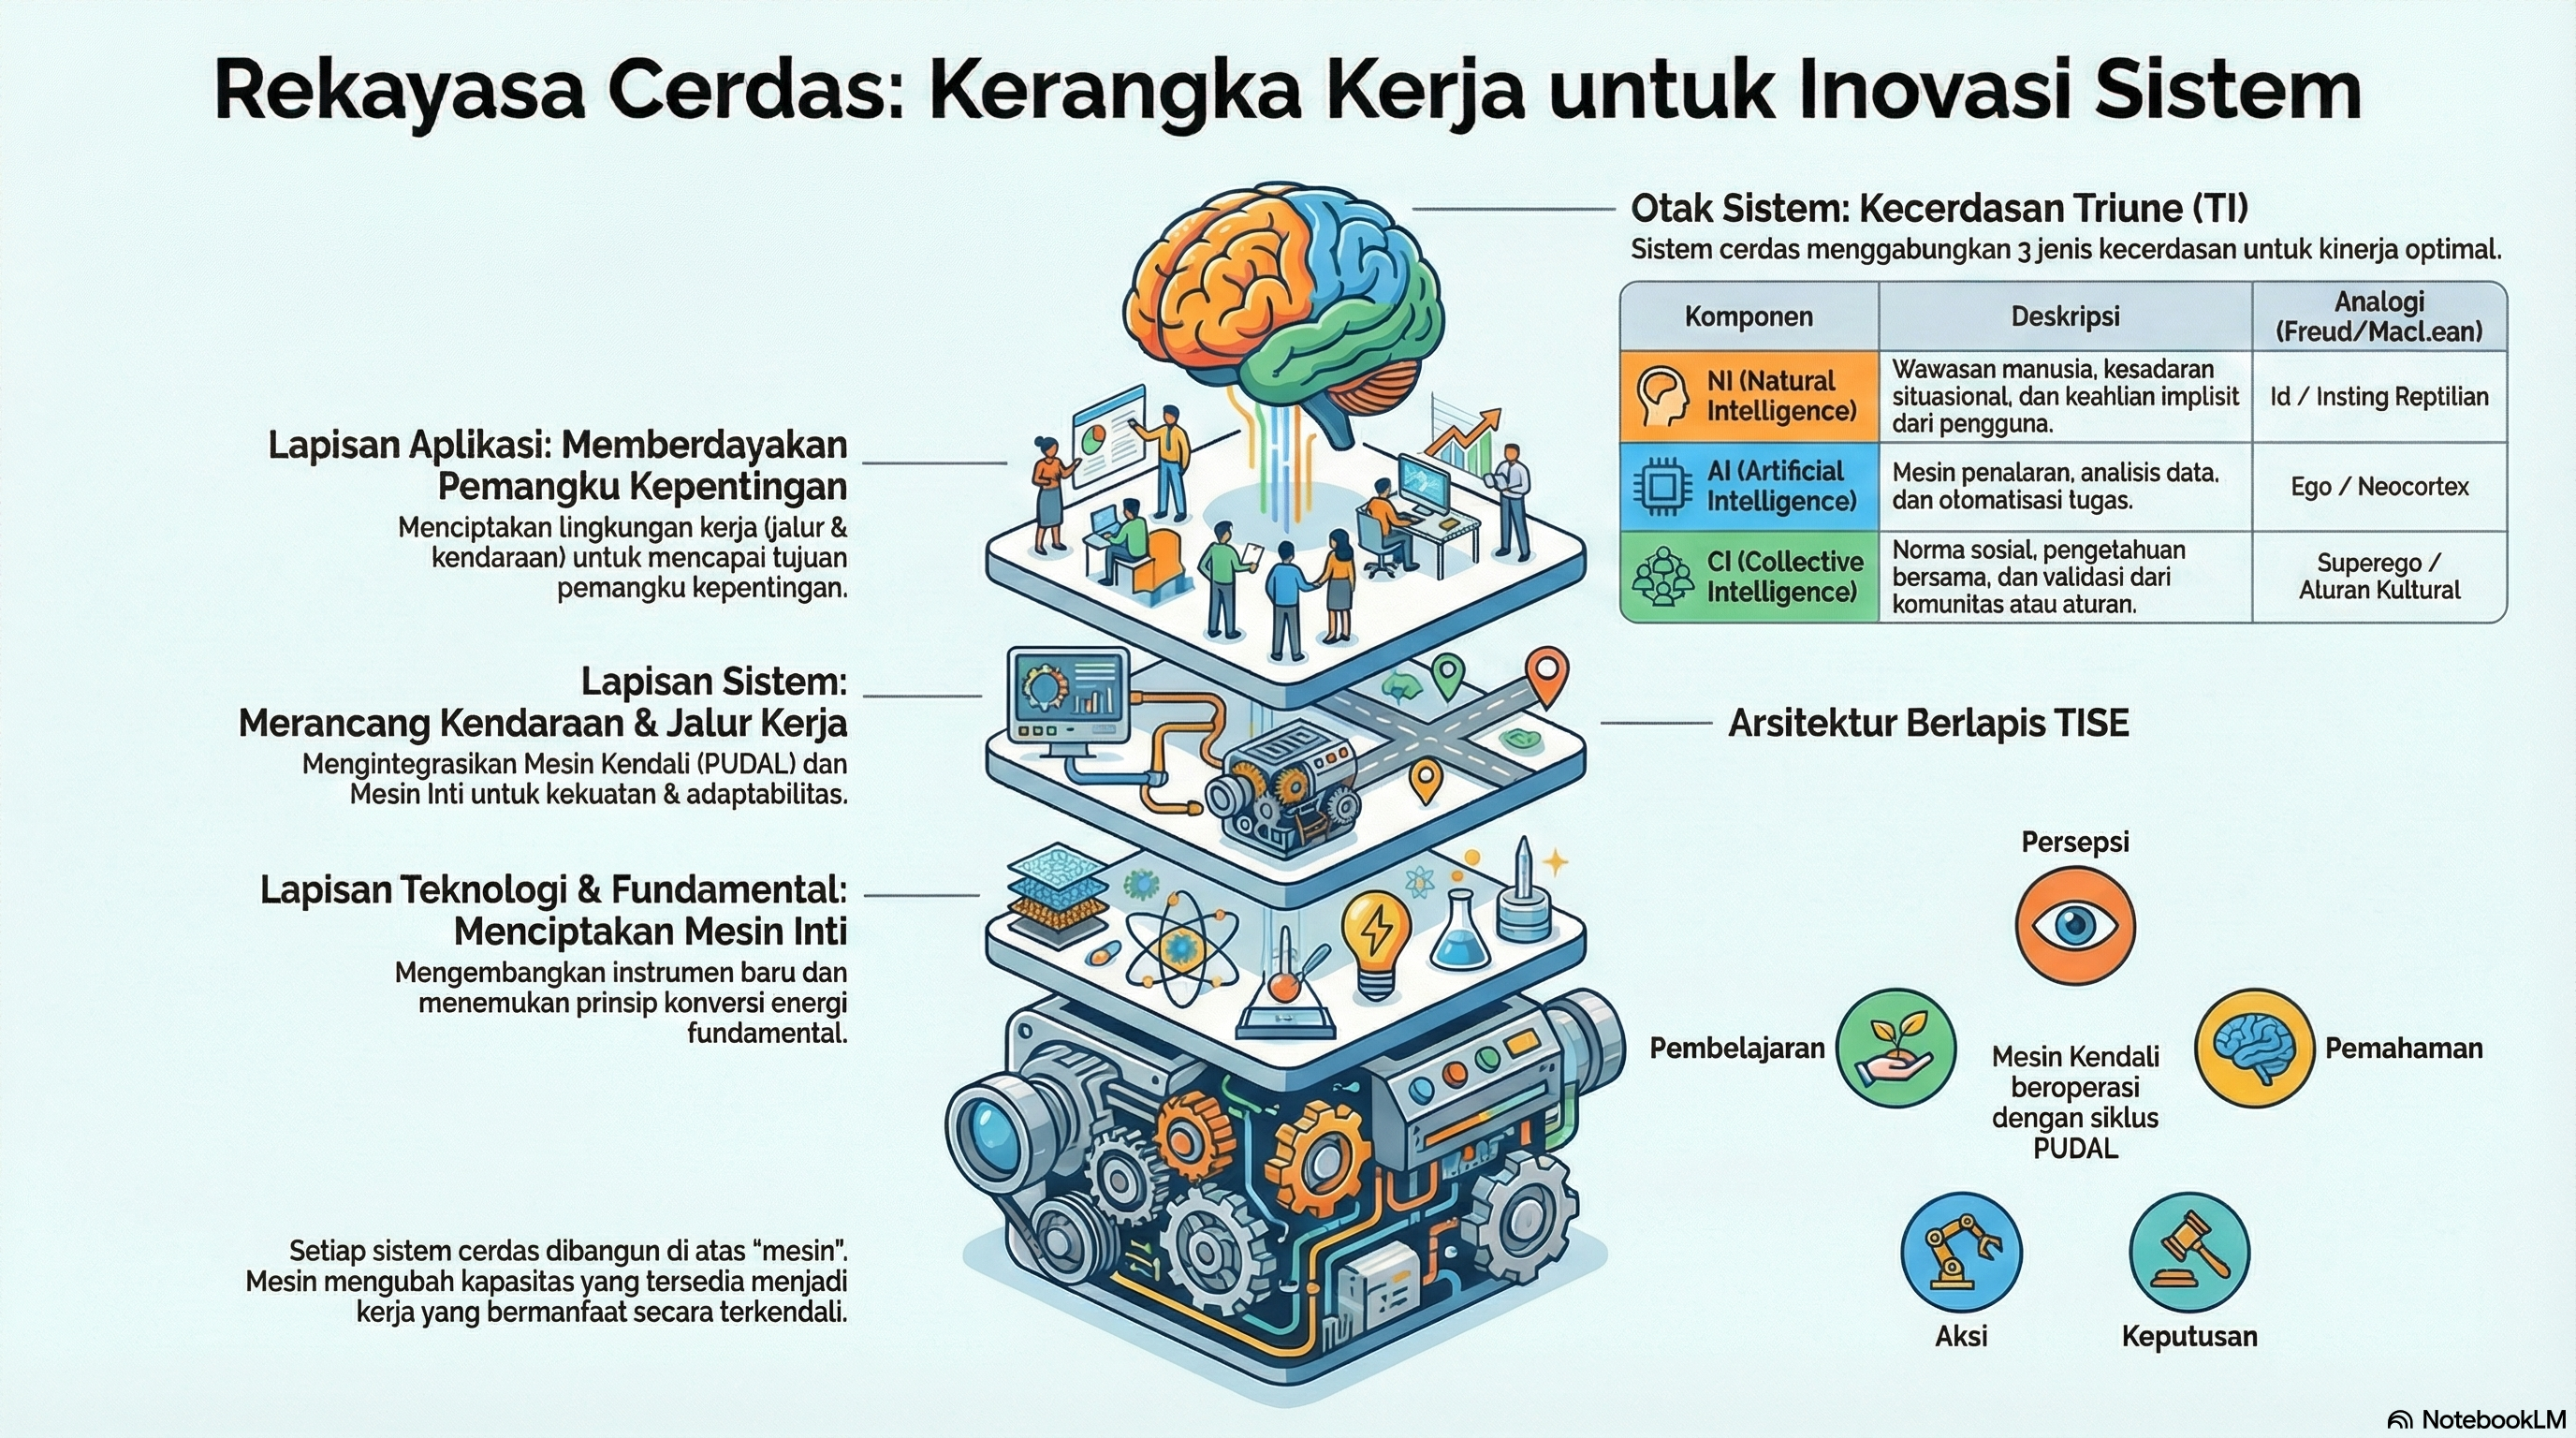
\includegraphics[keepaspectratio]{My_Concepts/../images/TISE.png}}

}

\caption{TISE}

\end{figure}%

Konsep saya tentang ``Mahakarya Rekayasa'' melampaui artefak teknis
belaka; ia adalah sebuah sistem sosio-teknis yang dirancang untuk
pemberdayaan kolektif. ``Masalah terbesar umat manusia''---kemiskinan,
konflik, degradasi lingkungan---pada intinya adalah krisis koordinasi
dan krisis makna. Untuk mengerahkan 8 miliar penduduk bumi, kita harus
terlebih dahulu memahami dan menyelaraskan tiga komponen fundamental
dari kecerdasan kolektif kita. Arsitektur konseptual ini saya sebut
sebagai \textbf{Triune Intelligence (Kecerdasan
Tripartit)}.\textsuperscript{3}

\begin{enumerate}
\def\labelenumi{\arabic{enumi}.}
\item
  \textbf{Hati (Kecerdasan Manusia / \emph{Homocordium}):} Ini adalah
  \textbf{Axiological Intelligence (AQ)} kolektif
  kita.\textsuperscript{2} ``Hati'', yang berasal dari \emph{Homo}
  (manusia) dan \emph{Cor} (hati) \textsuperscript{3}, adalah kompas
  nilai dan moral, ``mengapa'' di balik semua tindakan kita. Ia adalah
  sumber empati, etika, dan tujuan yang mendefinisikan ``masalah
  terbesar'' apa yang \emph{layak} untuk dipecahkan. Tanpa ``hati'' yang
  selaras, ``mahakarya'' apa pun akan menjadi optimasi tanpa jiwa. Kunci
  untuk pemberdayaan kolektif terletak pada \textbf{Komunikasi
  Interpersonal dan Publik}, yang merupakan proses di mana kita
  menyelaraskan \emph{Homocordium} kita.
\item
  \textbf{Pikiran (Kecerdasan Buatan / \emph{Homodeus}):} Ini adalah
  \textbf{Synergistic Practical Intelligence (PI-A)}
  \textsuperscript{2}, simbiosis manusia-AI. ``Pikiran'' adalah
  ``bagaimana'' teknisnya. Artificial Intelligence, seperti yang
  disarankan dalam petunjuk, adalah fasilitator \emph{par excellence}.
  Ia mampu menerjemahkan miliaran bahasa secara \emph{real-time} dan
  mengelola data dalam skala yang tak terbayangkan. Namun, AI hanyalah
  ``Instrumen Cerdas'' atau ``Juru Tulis Cerdas'' \textsuperscript{1};
  manusialah yang harus menggunakan \textbf{PI-A} untuk
  \emph{mengarahkan} AI, menerapkan penalaran logis, dan mengorkestrasi
  alur kerja yang kompleks untuk memecahkan masalah.
\item
  \textbf{Tenaga (Kecerdasan Alam / \emph{Natural Intelligence}):} Ini
  adalah ``apa'' yang kita gunakan---energi dan materi fundamental alam
  semesta.\textsuperscript{3} ``Tenaga'' 8 miliar manusia adalah ``Human
  Energon'' (waktu, fokus, kreativitas) \textsuperscript{5}; ``tenaga''
  planet adalah ``Environmental Energon''.\textsuperscript{3} Mahakarya
  Rekayasa harus ditenagai oleh \textbf{CORE Engine}
  \textsuperscript{5}, sebuah mesin konseptual yang mengelola ``tenaga''
  ini secara holistik melalui \textbf{PSKVE Engine} (Product, Service,
  Knowledge, Value, Environmental).\textsuperscript{3} Ini memastikan
  bahwa solusi kita berkelanjutan dan tidak menciptakan krisis baru
  dengan mengorbankan satu dimensi (misalnya Lingkungan) untuk dimensi
  lain (misalnya Nilai/Value).
\end{enumerate}

Oleh karena itu, Mahakarya Rekayasa Sistem dan TI di era AI bukanlah AI
super yang memecahkan masalah \emph{untuk} kita. Mahakarya itu adalah
\textbf{sistem TISE global} yang berfungsi sebagai platform Komunikasi
Publik, yang memungkinkan 8 miliar ``Protagonis-Penulis''
\textsuperscript{1} untuk menyelaraskan Hati (AQ) mereka, memperkuat
Pikiran (PI-A) mereka, dan mengelola Tenaga (PSKVE) mereka secara
bijaksana untuk berkolaborasi dalam ko-kreasi narasi kolektif umat
manusia.

\begin{quote}
\begin{quote}
\begin{quote}
\begin{quote}
\begin{quote}
\begin{quote}
\begin{quote}
7b0dbeadbf3074b08f16c9e765eb9abf42d8112d
\end{quote}
\end{quote}
\end{quote}
\end{quote}
\end{quote}
\end{quote}
\end{quote}

\bookmarksetup{startatroot}

\chapter{UAS-2 My Opinions}\label{uas-2-my-opinions}

\bookmarksetup{startatroot}

\chapter{\textless\textless\textless\textless\textless\textless\textless{}
HEAD}\label{head}

\bookmarksetup{startatroot}

\chapter{UAS-2 My Opinions}\label{uas-2-my-opinions-1}

\begin{quote}
\begin{quote}
\begin{quote}
\begin{quote}
\begin{quote}
\begin{quote}
\begin{quote}
7b0dbeadbf3074b08f16c9e765eb9abf42d8112d
\end{quote}
\end{quote}
\end{quote}
\end{quote}
\end{quote}
\end{quote}
\end{quote}

My Opinions: Sintesis Krisis, Komunikasi, dan Teknologi 1. Teknologi
Tanpa Komunikasi adalah Investasi yang Sia-sia Menurut pendapat saya,
banyak proyek infrastruktur air bersih gagal bukan karena teknologinya
(STI) tidak mumpuni, melainkan karena kegagalan komunikasi
interpersonal. Kita sering terjebak pada pemikiran bahwa menyediakan
sensor IoT atau aplikasi monitoring sudah cukup. Padahal, tanpa
komunikasi yang mengedepankan Local Framing, masyarakat mungkin akan
merasa terasing atau bahkan menolak teknologi tersebut karena dianggap
asing bagi budaya mereka. Teknologi harus berfungsi sebagai pendukung
(enabler) bagi hubungan antarmanusia, bukan penggantinya.

\textless\textless\textless\textless\textless\textless\textless{} HEAD
2. Transparansi Data adalah Bentuk Advokasi Publik yang Paling Jujur
Saya berpendapat bahwa dalam Komunikasi Publik, kejujuran data yang
didorong oleh STI adalah senjata terkuat. Seringkali data mengenai
sanitasi disembunyikan atau ``dipercantik'' demi citra politik. Dengan
sistem informasi yang terdesentralisasi (seperti penggunaan blockchain
atau database publik yang transparan), publik dapat memiliki kontrol
sosial. Pendapat saya adalah STI harus digunakan untuk memberikan
``suara'' bagi angka-angka statistik tersebut, sehingga krisis air tidak
lagi dianggap sebagai angka abstrak, melainkan urgensi nyata yang
menuntut tanggung jawab pemerintah.

\bookmarksetup{startatroot}

\chapter{3. Urgensi Desain Sistem yang Human-Centric (Berpusat pada
Manusia) Melihat target SDG 6 tahun 2030, pendapat saya adalah kita
membutuhkan pergeseran paradigma dalam pengembangan Sistem Teknologi
Informasi. Pengembang sistem (seperti kita di jurusan STI) tidak boleh
hanya memikirkan efisiensi algoritma atau skalabilitas database, tetapi
harus memikirkan User Experience (UX) bagi masyarakat pelosok. Jika
aplikasi pelaporan air sulit digunakan oleh orang awam, maka feedback
loop komunikasi interpersonal akan terputus. Keberhasilan teknologi
diukur dari seberapa mampu ia memfasilitasi komunikasi yang inklusif
bagi mereka yang paling
membutuhkan.}\label{urgensi-desain-sistem-yang-human-centric-berpusat-pada-manusia-melihat-target-sdg-6-tahun-2030-pendapat-saya-adalah-kita-membutuhkan-pergeseran-paradigma-dalam-pengembangan-sistem-teknologi-informasi.-pengembang-sistem-seperti-kita-di-jurusan-sti-tidak-boleh-hanya-memikirkan-efisiensi-algoritma-atau-skalabilitas-database-tetapi-harus-memikirkan-user-experience-ux-bagi-masyarakat-pelosok.-jika-aplikasi-pelaporan-air-sulit-digunakan-oleh-orang-awam-maka-feedback-loop-komunikasi-interpersonal-akan-terputus.-keberhasilan-teknologi-diukur-dari-seberapa-mampu-ia-memfasilitasi-komunikasi-yang-inklusif-bagi-mereka-yang-paling-membutuhkan.}

Bagiamana menjaadi menarik? \href{./Interesting.mp4}{Menjadi Menarik}

Ini adalah opini tentang \textbf{perubahan drastis} yang harus
diterapkan dalam pembelajaran ilmu rekayasa di era Kecerdasan Buatan
(Artificial Intelligence/AI), dengan mengusulkan \textbf{VALORAIZE
Learning} sebagai solusi untuk mentransformasi ruang kelas menjadi
miniatur lingkungan kerja profesional.

\textbf{Transformasi Pendidikan Rekayasa di Era AI: Dari Pembelajaran
Hafalan ke Penciptaan Nilai}

\begin{figure}[H]

{\centering \pandocbounded{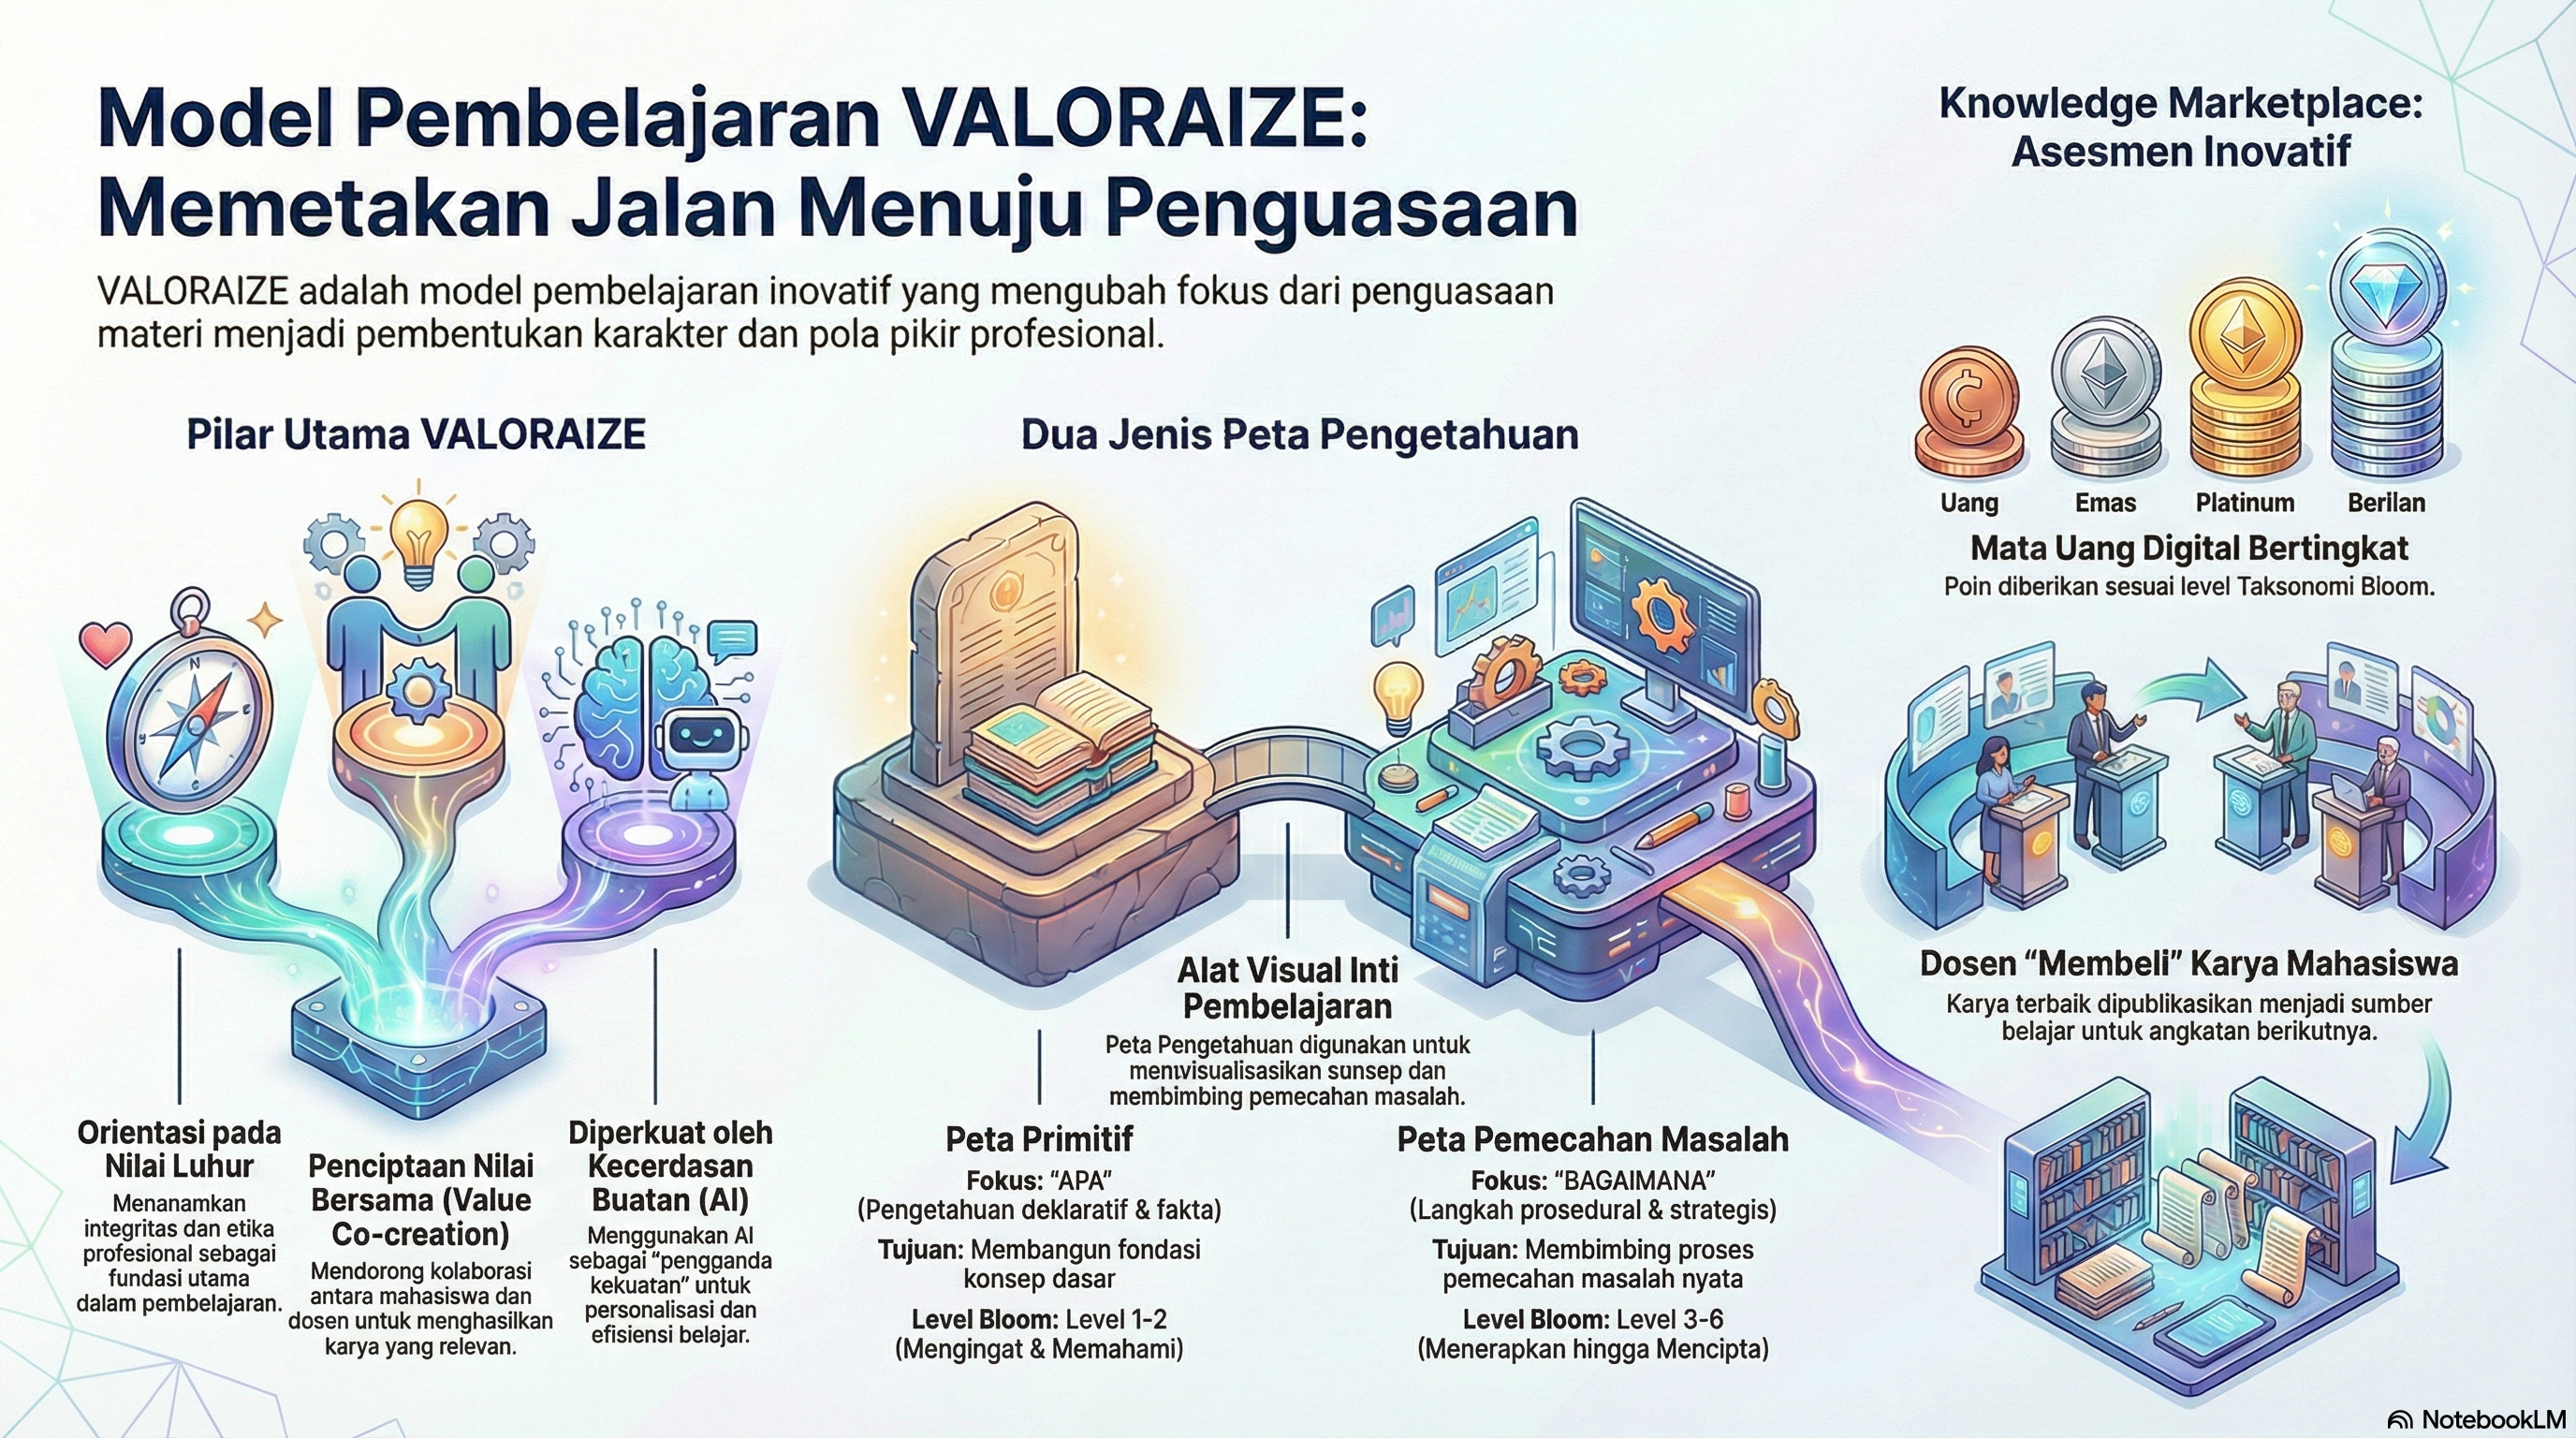
\includegraphics[keepaspectratio]{My_Opinions/../images/valorize.png}}

}

\caption{Valorize Learning}

\end{figure}%

\section{I. Krisis Model Konvensional di Tengah Supremasi
AI}\label{i.-krisis-model-konvensional-di-tengah-supremasi-ai}

Pembelajaran ilmu rekayasa dihadapkan pada pergeseran paradigma yang
fundamental dan \textbf{berubah drastis}. Akselerasi kemampuan
teknologi, terutama dalam domain Kecerdasan Buatan (AI), telah memicu
krisis naratif yang mendalam, di mana keunggulan manusia dipertanyakan.

Model pembelajaran konvensional---yang menekankan kuliah, penguasaan
\textbf{pengetahuan deklaratif} (fakta dan definisi), dan \textbf{ujian
tradisional}---\textbf{tidak lagi efektif}. Hal ini disebabkan karena
AI, khususnya Large Language Models (LLMs), telah mencapai kesempurnaan
dalam mode berpikir \textbf{``paradigmatik''} (logika, formal,
kategorisasi, dan komputasi) pada skala dan kecepatan yang jauh
melampaui kapasitas manusia.

Konsekuensinya, mahasiswa dapat menggunakan AI sebagai \textbf{``Juru
Tulis Cerdas''} (\emph{Smart Scribe}) atau \textbf{``pengganda
kekuatan''} (\emph{power multiplier}) untuk \textbf{menjawab ujian
dengan benar tanpa menguasai materi secara mendalam}. Kekuatan AI dalam
mengorganisir informasi dan mengeksekusi tugas-tugas kompleks
membebaskan kapasitas kognitif manusia. Jika penilaian masih berfokus
pada jawaban akhir (yang dapat dihitung oleh mesin), maka tujuan belajar
yang sejati---yaitu kebijaksanaan, tujuan, dan kemampuan untuk menulis
kisah hidup yang bermakna---terkikis.

Oleh karena itu, rekayasa pendidikan harus bergeser dari tujuan
konvensional rekayasa yang berfokus pada ``menyelesaikan masalah''
menuju visi yang lebih luhur: \textbf{``memberdayakan pemangku
kepentingan manusia untuk menyelesaikan masalah mereka sendiri''}.

\section{II. Ruang Kelas sebagai Lingkungan Kerja
Rekayasawan}\label{ii.-ruang-kelas-sebagai-lingkungan-kerja-rekayasawan}

Pergeseran ini menuntut transformasi radikal di mana \textbf{ruang kelas
menjadi miniatur lingkungan kerja rekayasawan}. Mahasiswa tidak boleh
lagi hanya menjadi \textbf{penerima pasif} atau ``Aktor/Musisi yang
mengeksekusi bagiannya''. Sebaliknya, mereka \textbf{perlu mendapat
pengalaman dini sebagai rekayasawan} dengan mengambil peran sebagai
\textbf{``Protagonis-Penulis''} yang memiliki otoritas dan agensi atas
cerita mereka.

Dalam lingkungan rekayasa, tujuannya adalah merancang skema untuk
\textbf{ko-kreasi nilai} (\emph{value co-creation}), di mana para
pemangku kepentingan bertukar \textbf{energon} (kapasitas melakukan
usaha---seperti waktu, tenaga, dan pengetahuan) untuk memperoleh apa
yang dibutuhkan. Inovasi adalah skema baru dalam merangkai berbagai
elemen artefak untuk menjadi sebuah lingkungan kerja yang berkelanjutan
(\emph{sustainable}).

\section{III. VALORAIZE Learning: Model Ko-Kreasi Nilai di
Kelas}\label{iii.-valoraize-learning-model-ko-kreasi-nilai-di-kelas}

Untuk memfasilitasi transformasi ini, \textbf{pembelajaran VALORAIZE}
diusulkan. Filosofi utama VALORAIZE adalah \textbf{membawa simulasi
profesi ke dalam ruang kelas} dan mengalihkan fokus dari penguasaan
materi belaka ke \textbf{pembentukan sosok, karakter, dan pola berpikir
profesional} yang komprehensif.

Dalam model ini, mahasiswa belajar menjadi sosok rekayasawan melalui
proses berikut:

\subsection{1. Penguasaan Materi melalui Penciptaan Artefak
Pengetahuan}\label{penguasaan-materi-melalui-penciptaan-artefak-pengetahuan}

Mahasiswa memproduksi \textbf{Produk Pengetahuan} (artefak pembelajaran)
yang merepresentasikan pemahaman mendalam mereka dan memiliki
\textbf{nilai nyata} yang dapat dimanfaatkan oleh orang lain. Ini adalah
praktik otentik penguasaan materi yang dapat divalidasi:

\begin{itemize}
\tightlist
\item
  \textbf{Pembuatan Peta Pengetahuan Primitif:} Mahasiswa
  \textbf{mempraktekkan penguasaan materi} dengan mengorganisir
  \textbf{pengetahuan deklaratif} (fakta dan definisi), berfokus pada
  ``Apa'' dari pengetahuan, dan umumnya menguji tingkat Mengingat dan
  Memahami (Level 1-2 Taksonomi Bloom).
\item
  \textbf{Penyusunan Peta Pengetahuan Aplikatif:} Mahasiswa
  \textbf{menyusun peta pengetahuan aplikatif} yang bersifat dinamis dan
  berorientasi proses. Peta ini berfokus pada ``Bagaimana'' dari
  pengetahuan, mengintegrasikan konsep dengan langkah-langkah
  prosedural. Peta ini dirancang untuk membimbing proses pemecahan
  masalah dan menguji kemampuan Menerapkan, Menganalisis, Mengevaluasi,
  hingga Menciptakan (Level 3-6 Bloom).
\end{itemize}

\subsection{2. Menjual di Pasar Pengetahuan (Knowledge
Marketplace)}\label{menjual-di-pasar-pengetahuan-knowledge-marketplace}

Penilaian diubah dari ujian pasif menjadi aktivitas ekonomi-intelektual
yang disebut \textbf{Knowledge Marketplace}. Model asesmen inovatif ini
dirancang untuk memberikan \textbf{``rasa menciptakan nilai''} kepada
mahasiswa.

\begin{itemize}
\tightlist
\item
  \textbf{Peran Mahasiswa dan Dosen:} Dosen bertindak sebagai
  \textbf{``Pencipta Kebutuhan''} dengan mengiklankan kebutuhan akan
  karya pengetahuan. Mahasiswa bertindak sebagai \textbf{``Pencipta
  Nilai''} dengan merespons melalui produksi artefak (peta pengetahuan).
\item
  \textbf{Mata Uang Pembelian:} Karya mahasiswa \textbf{dijual di pasar
  pengetahuan} untuk kemudian \textbf{dibeli dosen dengan berbagai jenis
  mata uang} digital berjenjang dan mata uang fiat:

  \begin{itemize}
  \tightlist
  \item
    \textbf{Mata uang digital} (Poin Uang, Poin Emas, Poin Platinum,
    Poin Berlian) terkait langsung dengan tingkat Taksonomi Bloom yang
    diuji dalam peta yang dibuat (Level 1-6).
  \item
    \textbf{Mata uang fiat} (misalnya, IDR, USD, EUR) dikaitkan dengan
    domain teknis spesifik untuk mendorong eksplorasi area tertentu.
  \end{itemize}
\end{itemize}

\subsection{3. Nilai Akhir Berbasis Portofolio Kekayaan
Rekayasawan}\label{nilai-akhir-berbasis-portofolio-kekayaan-rekayasawan}

Di akhir pembelajaran, nilai akhir (\emph{grade}) tidak lagi didasarkan
pada ujian tunggal, melainkan pada portofolio kekayaan yang telah
dikumpulkan, yang disebut \textbf{portofolio kekayaan rekayasawan}.

\begin{itemize}
\tightlist
\item
  \textbf{Pemberian Nilai Akhir (\emph{Grade}):} Total \textbf{``harta''
  terkumpul} (poin dan mata uang fiat) diindeks untuk \textbf{nilai
  akhir mata kuliah}.
\item
  \textbf{Manfaat Portofolio:} Portofolio ini tidak hanya menilai hasil
  (\emph{product}), tetapi juga \textbf{proses dan perjuangan} mahasiswa
  dalam menulis \textbf{Jurnal Pembelajar Reflektif}---mencakup
  perjuangan, alat yang dipakai, kegagalan, terobosan, dan pelajaran
  yang dipetik. Hal ini sejalan dengan tujuan TISE 2.0 untuk memastikan
  mahasiswa adalah \textbf{Protagonis-Penulis} yang memahami
  \emph{Penalaran Otobiografis} dan membangun narasi \emph{Agensi}
  pribadi mereka.
\end{itemize}

Pendekatan VALORAIZE ini secara struktural melindungi integritas
akademik dengan mengalihkan penekanan penilaian dari jawaban tunggal
menuju \textbf{bukti penguasaan materi yang otentik dan penciptaan nilai
kolektif}.
\textgreater\textgreater\textgreater\textgreater\textgreater\textgreater\textgreater{}
7b0dbeadbf3074b08f16c9e765eb9abf42d8112d

\bookmarksetup{startatroot}

\chapter{UAS-3 My Innovations}\label{uas-3-my-innovations}

\begin{figure}[H]

{\centering \pandocbounded{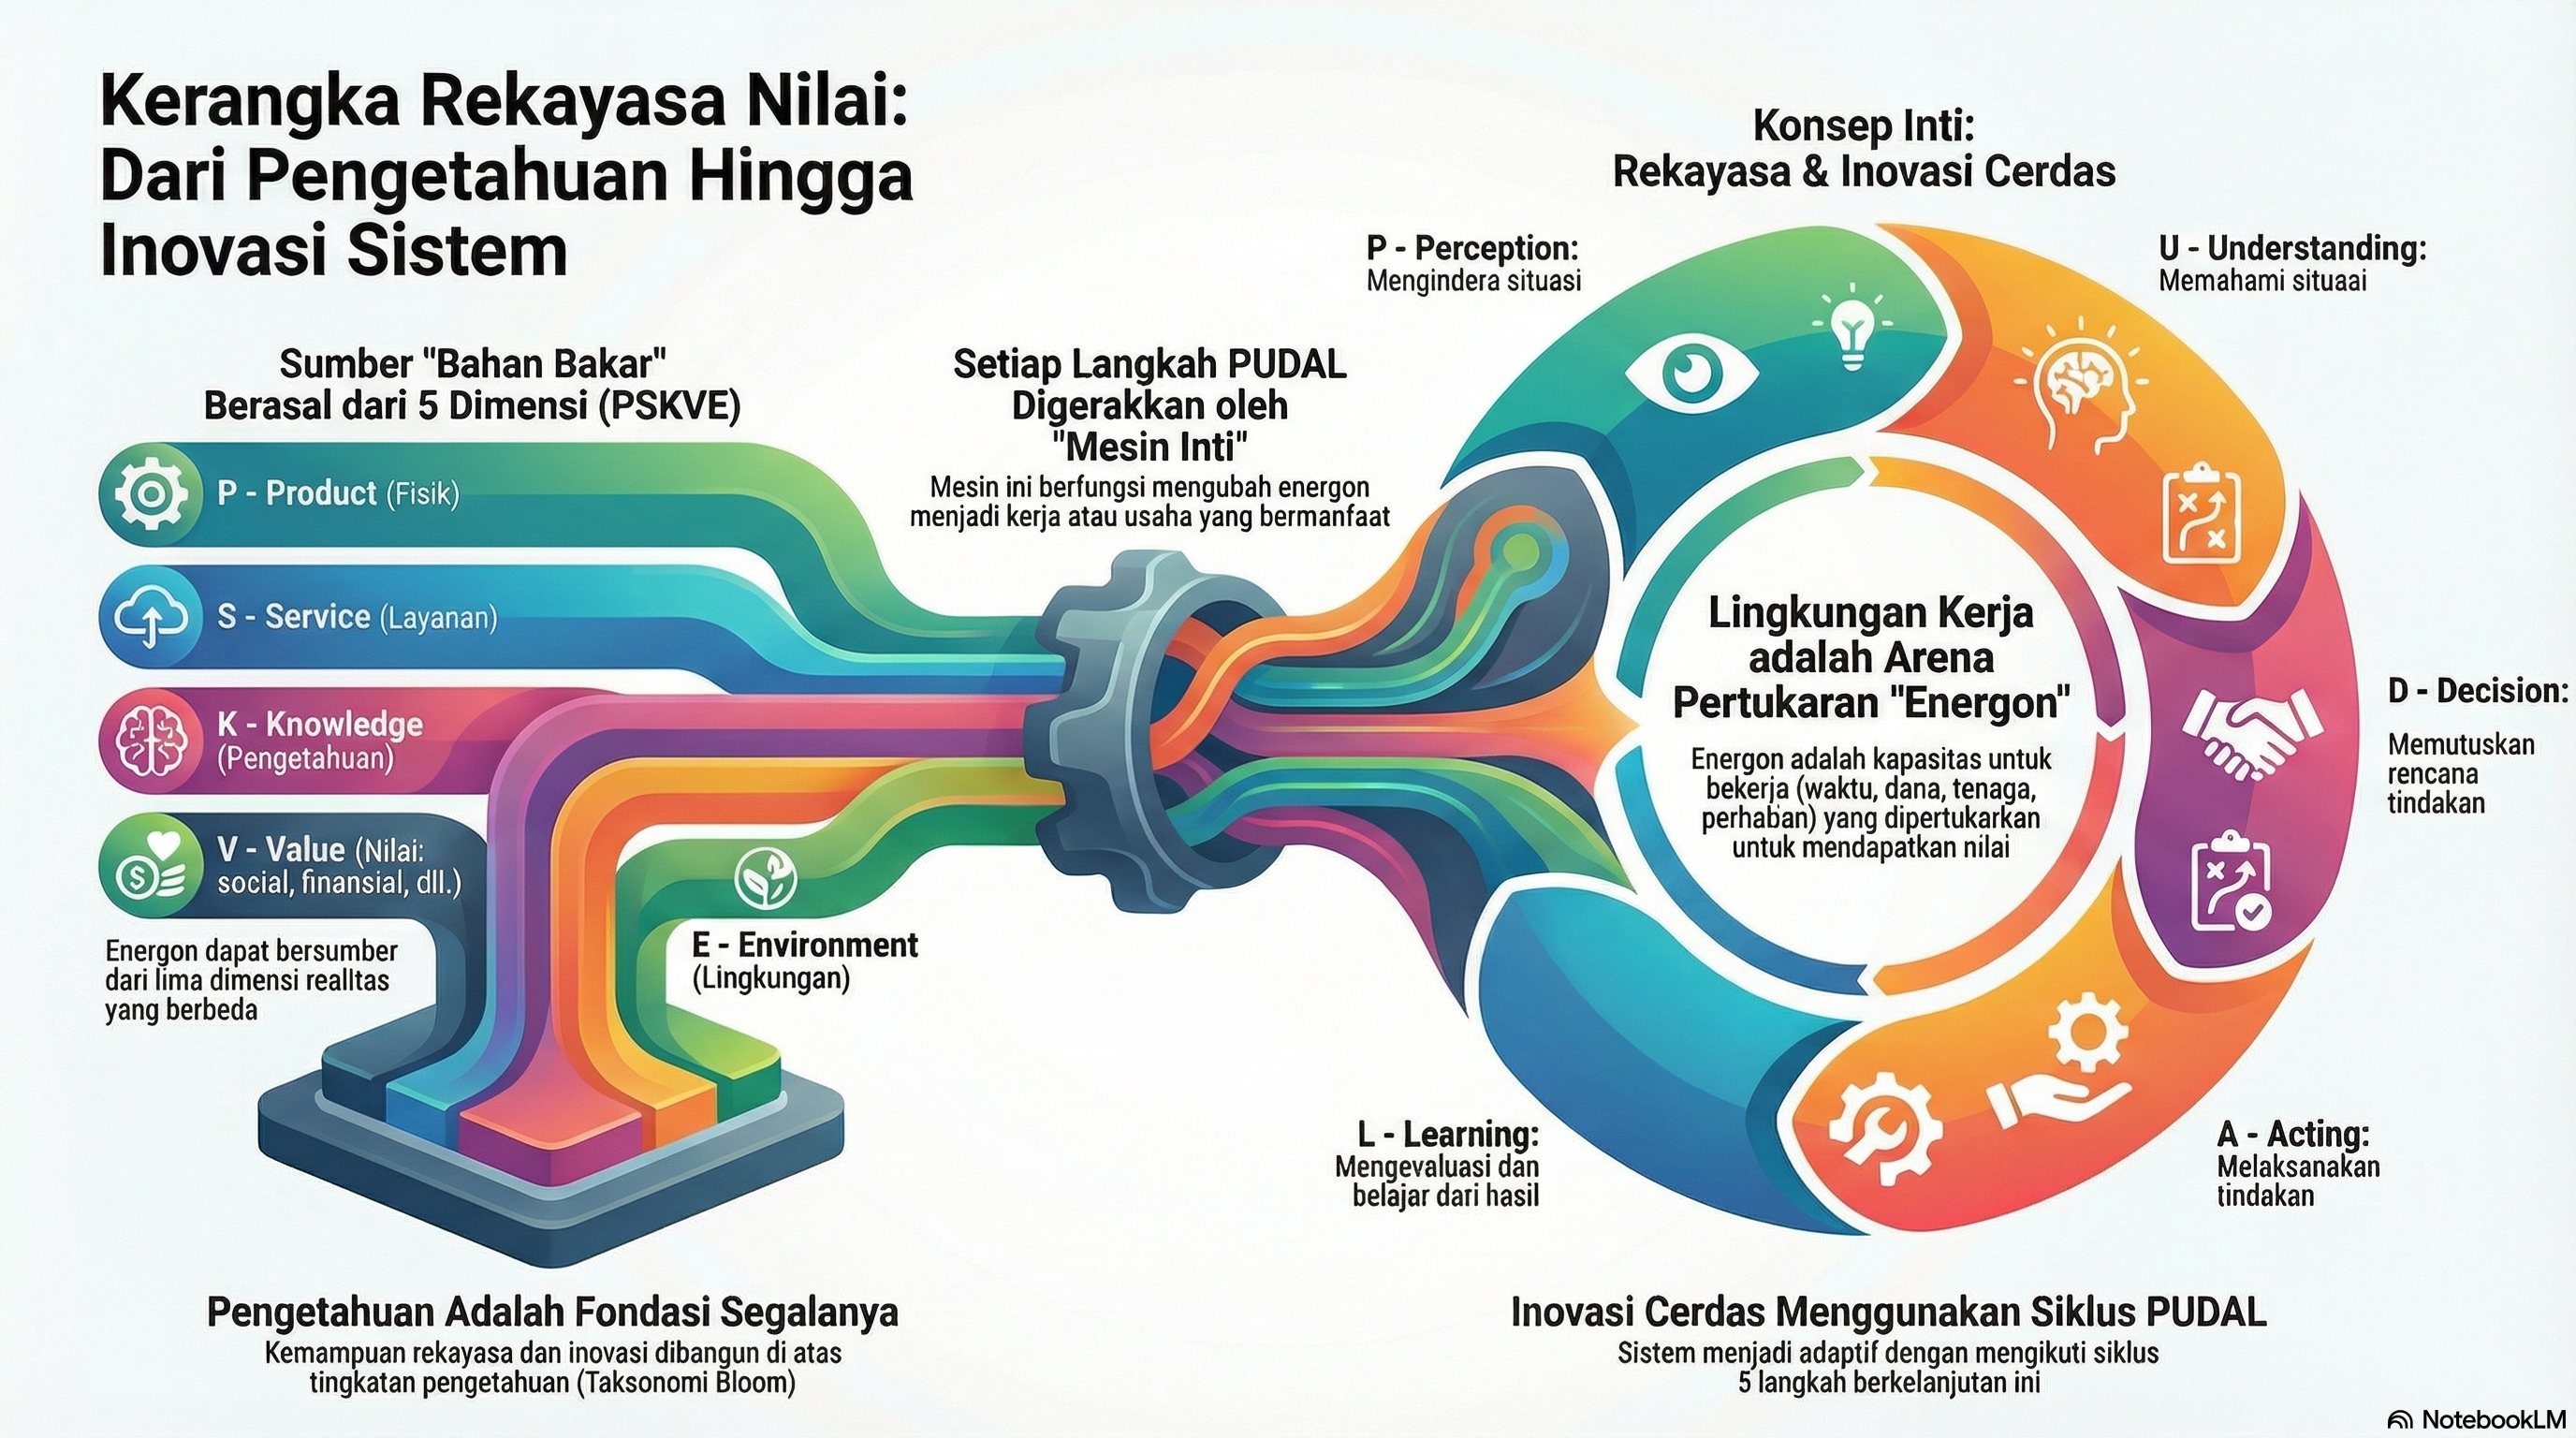
\includegraphics[keepaspectratio]{My_Innovations/../images/PUDAL.png}}

}

\caption{PUDAL}

\end{figure}%

\textbf{Judul: TISE 2.0: Arsitektur ``Teater Kerja'' Agentik}

Inovasi utama saya adalah pengembangan paradigma
\textbf{Triune-Intelligence Smart Engineering (TISE)}, dan evolusinya
dari TISE 1.0 ke TISE 2.0. TISE 1.0 berfokus pada perancangan
``Sub-Ruang'' atau ``Teater Kerja'' untuk orkestrasi tugas yang efisien,
guna menjembatani kesenjangan antara Titik A (saat ini) dan Titik B
(yang diinginkan) dalam Ruang PSKVE.\textsuperscript{1} TISE 2.0
mengambil arsitektur ini dan mengisinya dengan tujuan yang lebih tinggi:
ko-kreasi naratif dan pemberdayaan \textbf{Agensi}
\emph{stakeholder}.\textsuperscript{1}

``Teater kerja'' ini adalah implementasi teknis dari ``lingkungan'' yang
saya bahas di `My Opinions'. Ini adalah \textbf{Sub-Ruang PSKVE}
\textsuperscript{6} yang dirancang untuk memberdayakan rekayasawan
Sistem dan Teknologi Informasi dalam memfasilitasi pemecahan masalah
(\emph{Problem Solving}). Arsitektur operasionalnya terdiri dari
komponen-komponen berikut:

\begin{enumerate}
\def\labelenumi{\arabic{enumi}.}
\item
  \textbf{Stasion:} Ini adalah \emph{hub} fungsional dalam teater kerja
  di mana nilai diciptakan atau dipertukarkan. Dalam alegori ``The Helix
  Commute'', ini adalah ``Stasiun A (Ide)'' dan ``Stasiun B (Produk
  Selesai)''.\textsuperscript{5} Ini adalah titik-titik di mana ``PSKVE
  Energon'' ditransduksi (misalnya, `Human Energon' diubah menjadi
  `Product Energon').
\item
  \textbf{Kendaraan (Agen PUDAL):} Untuk bergerak di antara stasiun,
  \emph{stakeholder} membutuhkan ``kendaraan''. ``Kendaraan'' ini
  bukanlah perangkat fisik, melainkan \textbf{Agen Pemecah Masalah
  (Problem Solving Agent - PSA)} yang cerdas dan
  otonom.\textsuperscript{8} Arsitektur kognitif dari agen ini adalah
  sistem \textbf{PUDAL} (Perceive, Understand, Decision, Act,
  Learning-evaluating).\textsuperscript{3}
\item
  \textbf{Jaringan Rute Jalan (Siklus PUDAL/Problem Solving):}
  ``Kendaraan'' (Agen PUDAL) tidak bergerak secara acak; ia mengikuti
  ``jaringan rute jalan''. Rute ini adalah \textbf{Siklus 7-Langkah
  Pemecahan Masalah} (1. Identifikasi Masalah, 2. Picu/Trigger, 3.
  Kejadian/Event, 4. Baca STATUS, 5. Evaluasi, 6. Adaptasi, 7.
  Selesai/Lesson Learned).\textsuperscript{8} Siklus 7-Langkah ini
  adalah \emph{manifestasi eksternal} dan alur kerja terstruktur dari
  siklus kognitif PUDAL \emph{internal} yang sedang beraksi, memandu
  \emph{stakeholder} melalui proses pemecahan masalah yang adaptif dan
  iteratif.\textsuperscript{8}
\item
  \textbf{Teknologi CORE Engine (Mesin Energon):} ``Kendaraan'' (Agen
  PUDAL) membutuhkan tenaga. Tenaga ini disediakan oleh \textbf{CORE
  Engine}.\textsuperscript{6} CORE Engine adalah \textbf{Mesin Energon}
  \textsuperscript{5}, sebuah \emph{transducer} fundamental yang
  beroperasi dalam siklus empat langkah (Input, Encode, Decode, Output)
  \textsuperscript{6} untuk mengubah satu bentuk energi ke bentuk
  lainnya.
\item
  \textbf{Fundamental Riset PSKVE (Bahan Bakar):} CORE Engine tidak
  menciptakan energi; ia mengubahnya. ``Bahan bakar'' untuk mesin ini
  berasal dari \textbf{Fundamental Riset PSKVE}.\textsuperscript{3}
  Riset fundamental inilah yang menemukan prinsip-prinsip konversi
  ``Energon'' (misalnya, `Human Energon' menjadi `Knowledge Energon',
  atau `Economic Energon' menjadi `Service Energon').\textsuperscript{5}
  Prinsip-prinsip ini kemudian digunakan oleh CORE Engine untuk
  menghasilkan ``Working Energon'' yang menggerakkan Agen
  PUDAL.\textsuperscript{7}
\end{enumerate}

Singkatnya, inovasi TISE 2.0 adalah arsitektur \emph{full-stack} untuk
pemberdayaan: dimulai dari \textbf{Riset PSKVE} (bahan bakar/prinsip),
ditenagai oleh \textbf{CORE Engine} (mesin/transducer), dieksekusi oleh
\textbf{Kendaraan PUDAL} (agen/kognisi), yang berjalan di atas
\textbf{Rute Siklus 7-Langkah} (proses/alur kerja), untuk memindahkan
\emph{stakeholder} antar \textbf{Stasiun} (tujuan/nilai), di dalam
\textbf{Teater Kerja TISE 2.0} (lingkungan pemberdayaan naratif).

\bookmarksetup{startatroot}

\chapter{UAS-4 My Knowledge}\label{uas-4-my-knowledge}

\textbf{VALORISE dan Penyelesaian Paradoks Pendidikan Rekayasa}

\begin{figure}[H]

{\centering \pandocbounded{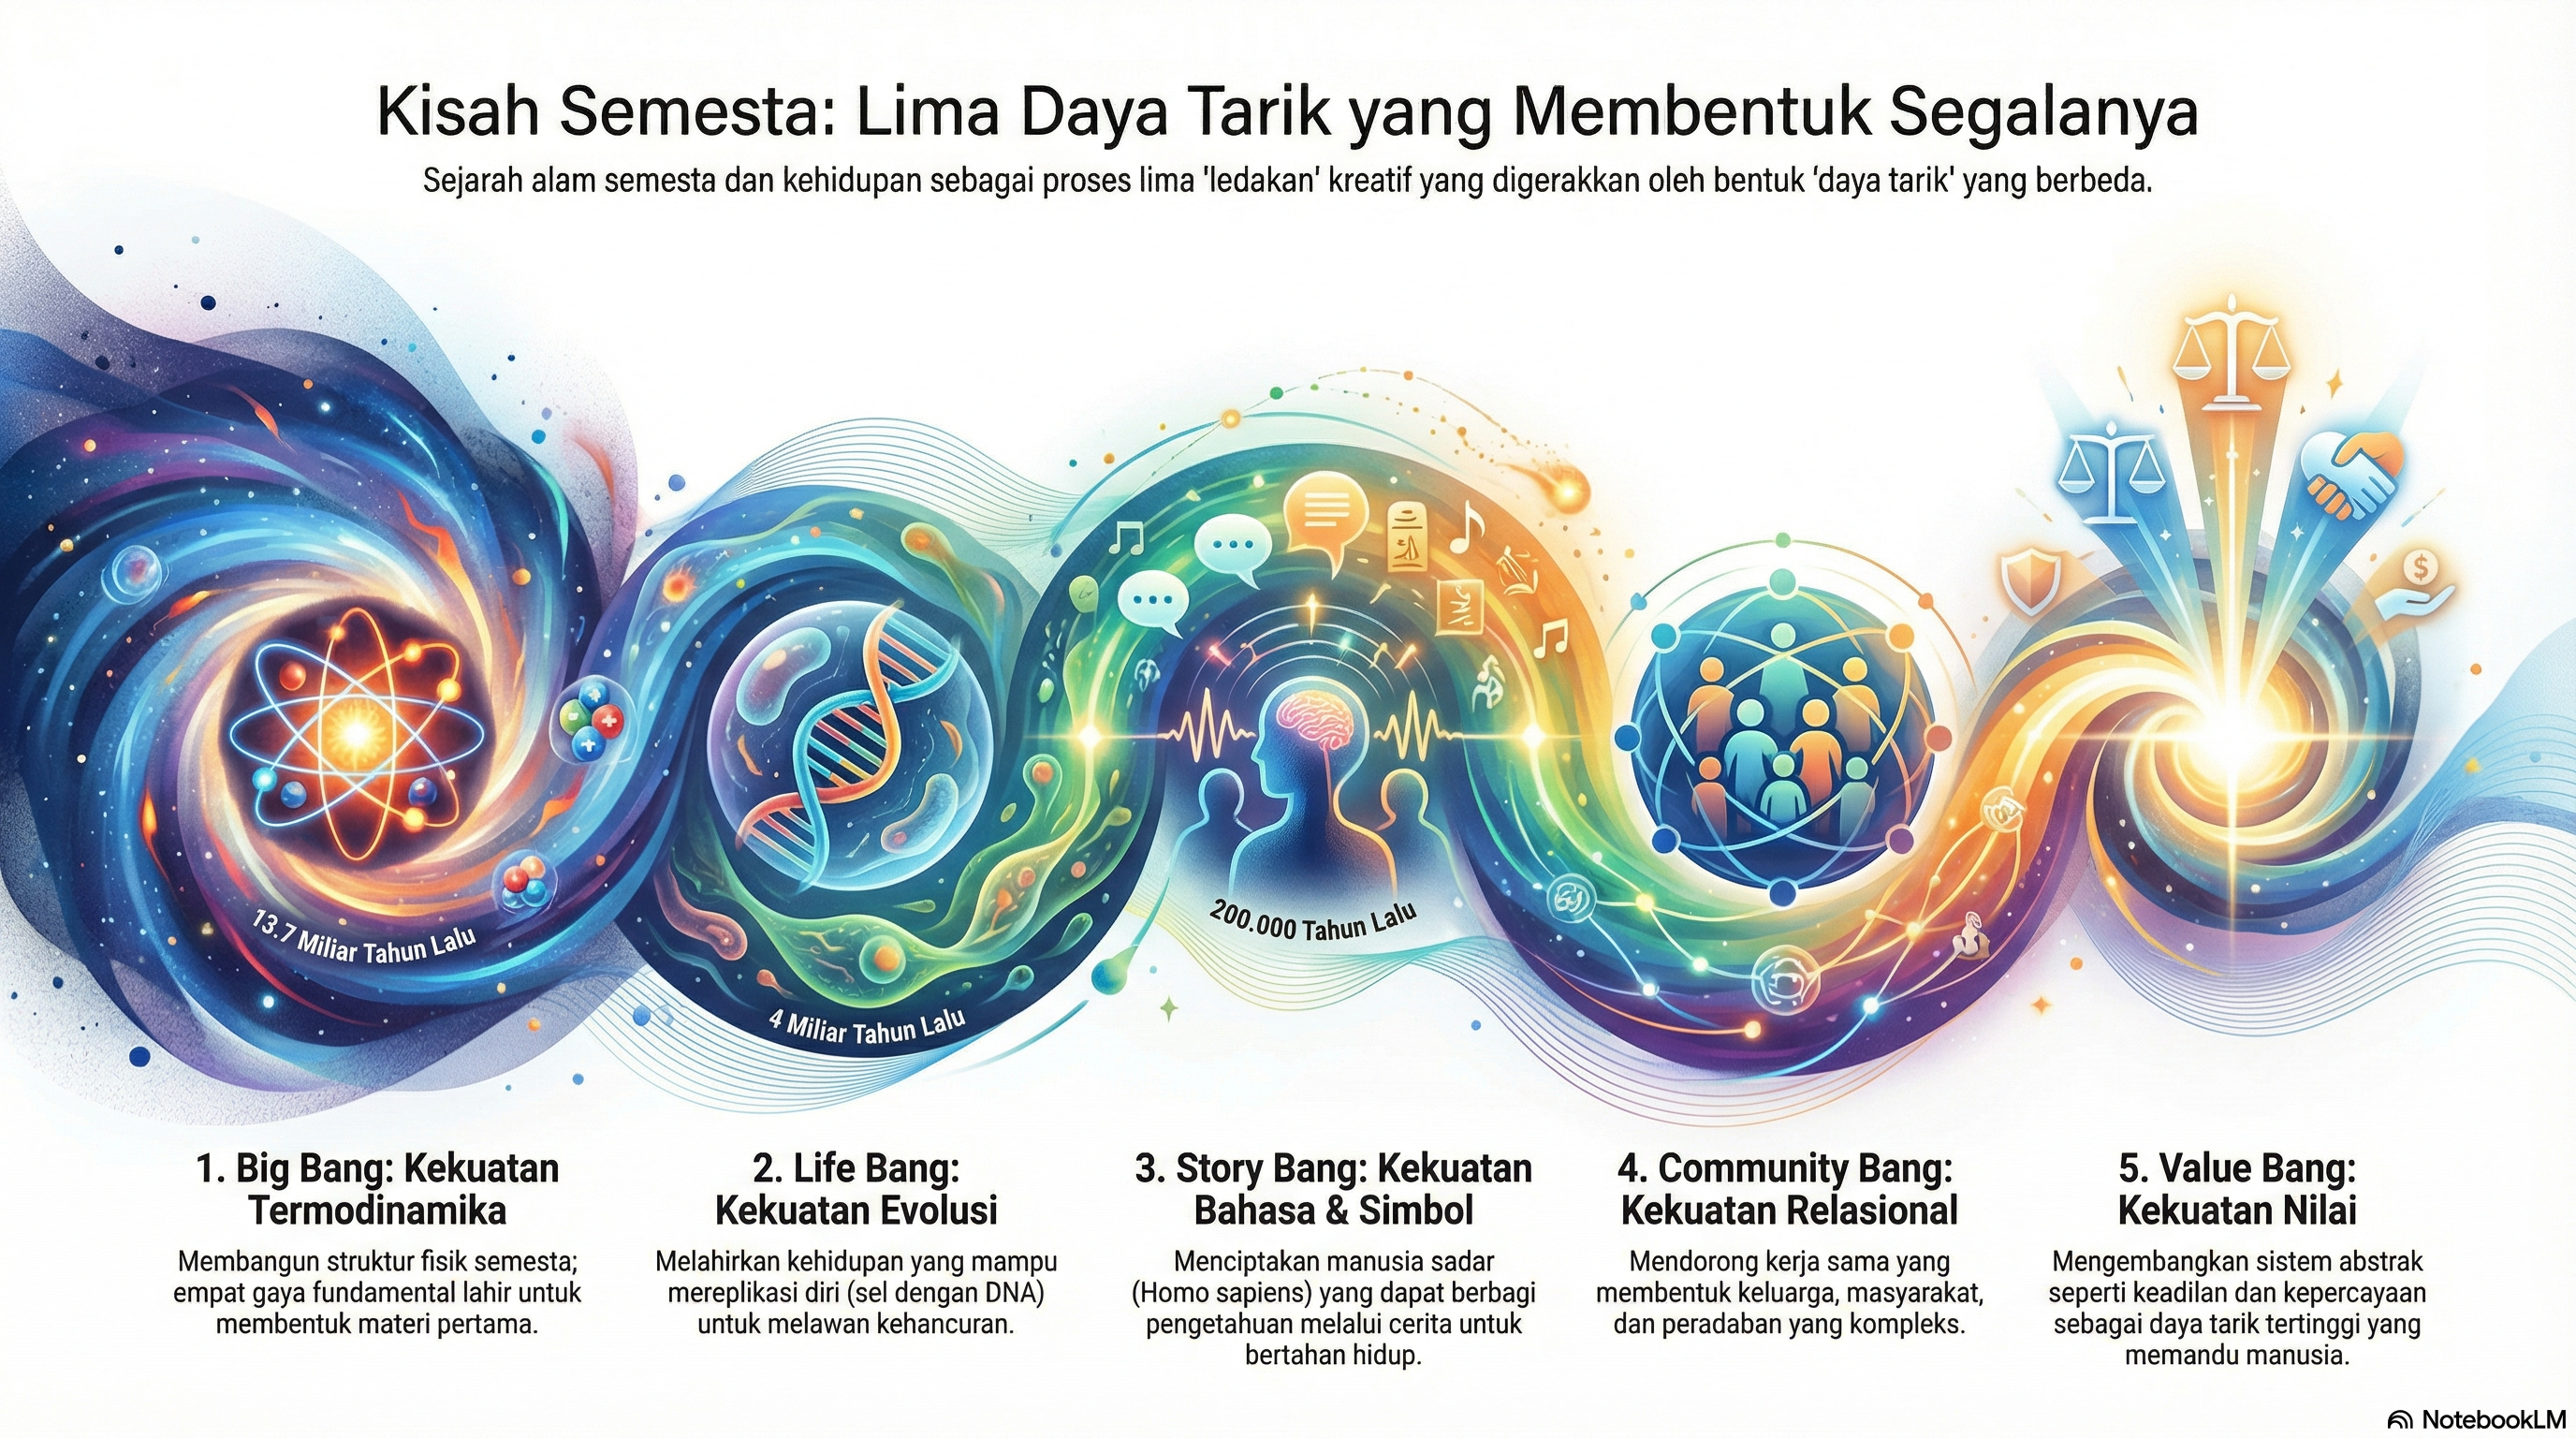
\includegraphics[keepaspectratio]{My_Knowledge/../images/5forces.png}}

}

\caption{Valorize Learning}

\end{figure}%

Untuk mengajarkan paradigma TISE yang kompleks, metode pedagogis
konvensional tidak memadai. Oleh karena itu, saya mengembangkan
\textbf{VALORISE}. Ini adalah metodologi pedagogis TISE yang dirancang
untuk menyelesaikan ``Paradoks Pendidikan Ilmu Rekayasa''.

Paradoksnya adalah ini: Bagaimana kita bisa menggunakan alat
pemberdayaan mesin yang kuat (seperti AI generatif) tanpa
\emph{melemahkan} pemberdayaan manusia (Agensi, \emph{Self-Authorship})?
Jika AI memberi siswa semua jawaban, mesin menjadi lebih pintar, tetapi
siswa tidak.\textsuperscript{10} Ini adalah kegagalan pedagogis.

VALORISE menyelesaikan ini dengan dua komponen utama: struktur kurikulum
dan desain agen pedagogis.

\begin{enumerate}
\def\labelenumi{\arabic{enumi}.}
\item
  \textbf{Struktur Kurikulum (Peta ASTF):}

  \begin{itemize}
  \item
    \textbf{Peta Pengetahuan:} Ini bukanlah daftar topik acak. Ia adalah
    \textbf{Lapisan Fundamental (F) dan Teknologi (T)} dari
    \textbf{Arsitektur ASTF}.\textsuperscript{3} Siswa harus terlebih
    dahulu memahami prinsip-prinsip dasar: fisika ``Energon''
    \textsuperscript{4}, anatomi mesin PSKVE \textsuperscript{3}, dan
    psikologi TISE 2.0 (AQ, Agensi, Penebusan).\textsuperscript{1}
  \item
    \textbf{Peta Aplikasi:} Ini adalah \textbf{Lapisan Aplikasi (A) dan
    Sistem (S)} dari \textbf{ASTF}.\textsuperscript{3} Siswa harus
    menerapkan ``peta pengetahuan'' mereka untuk merancang dan membangun
    sistem nyata (artefak TISE) yang memecahkan masalah pemangku
    kepentingan yang nyata.\textsuperscript{10}
  \end{itemize}
\item
  \textbf{Proses Validasi (W-Model \& PICOC):}

  \begin{itemize}
  \item
    Pembelajaran TISE tidak linear; ia mengikuti proses
    \textbf{W-Model}.\textsuperscript{3} Siswa mulai di kiri atas
    (Aplikasi - masalah), turun ke kiri bawah (Fundamental - riset
    prinsip) untuk mengisi ``peta pengetahuan'' mereka. Kemudian, mereka
    naik di sisi kanan (F \(\rightarrow\) T \(\rightarrow\) S
    \(\rightarrow\) A) untuk membangun solusi di ``peta aplikasi''
    mereka.
  \item
    Untuk \emph{membuktikan} penguasaan, siswa harus menggunakan
    \textbf{PICOC Berlapis} (\emph{Layered PICOC}).\textsuperscript{3}
    Mereka harus membuat ``rantai bukti'' yang tak terputus, memvalidasi
    klaim mereka di setiap lapisan ASTF: \emph{Outcome} di lapisan F
    (prinsip baru terbukti), \emph{Outcome} di lapisan T (teknologi baru
    lebih efisien), \emph{Outcome} di lapisan S (sistem baru lebih
    andal), dan \emph{Outcome} di lapisan A (aplikasi baru lebih
    memuaskan pengguna).
  \end{itemize}
\item
  \textbf{Penyelesaian Paradoks (Pemihakan pada Pemberdayaan Manusia):}

  \begin{itemize}
  \item
    Inilah inti dari VALORISE. Agen PUDAL (PSA) yang membantu siswa
    belajar dirancang dengan \textbf{``Anti-Answer
    Constraint''}.\textsuperscript{10}
  \item
    Ini adalah pemihakan desain yang disengaja. \textbf{D-Agent}
    (\emph{Decision-making}) dari sistem PUDAL \emph{dilarang}
    memberikan jawaban yang efisien (pemberdayaan mesin). Sebaliknya, ia
    \emph{diwajibkan} secara etis dan pedagogis untuk memprioritaskan
    intervensi (\emph{scaffolding}) yang membangun \textbf{Agensi} dan
    \textbf{Self-Authorship} siswa (pemberdayaan
    manusia).\textsuperscript{2}
  \item
    Agen VALORISE tidak akan menjawab, ``Apa jawabannya?'' Sebaliknya,
    ia akan merespons dengan \emph{prompt} reflektif TISE 2.0
    \textsuperscript{1}: ``Itu tantangan yang menarik. Apa yang telah
    Anda coba? Kekuatan apa dari diri Anda yang dapat Anda gunakan untuk
    meresponsnya?''
  \end{itemize}
\end{enumerate}

Dengan demikian, VALORISE menggunakan AI bukan untuk menggantikan
pemikiran, tetapi untuk \emph{memprovokasi} \textbf{Penalaran
Otobiografis}, memaksa siswa untuk menjadi \textbf{Protagonis-Penulis}
dari pembelajaran mereka sendiri. Ini adalah pemihakan radikal, dan
perlu, pada pemberdayaan manusia di era AI.

\bookmarksetup{startatroot}

\chapter{UAS-5 My Professional
Reviews}\label{uas-5-my-professional-reviews}

Untuk melAkukan review, seperti pada
\href{../My_Personal_Reviews/Doc.5.Mengevaluasi-Esai-Berdasarkan-Rubrik.pdf}{pendekatan
AI}, kita membutuhkan rubrik

\bookmarksetup{startatroot}

\chapter{Summary}\label{summary}

In summary, this book has no content whatsoever.

\bookmarksetup{startatroot}

\chapter*{References}\label{references}
\addcontentsline{toc}{chapter}{References}

\markboth{References}{References}

\phantomsection\label{refs}




\end{document}
